\chapter{Uncertainty Propagation to Enable Uncertainty Impact Analysis}%
\label{ch:impactanalysis}%


In this chapter, we present the second Contribution \C{2}.
This contribution covers the third activity shown in \autoref{sec:overview:procedure}, i.e., the propagation of uncertainty.
We present means to model and analyze uncertainty in software architectures in order to enable the early assessment of the potential impact of uncertainty on confidentiality.

As motivated throughout this thesis, uncertainty can quickly become critical, especially regarding security-related properties like confidentiality.
For proactive decision-making as implied by \emph{Privacy by Design} \cite{schaar_privacy_2010} and adaptation to a changing environment, uncertainty should be analyzed as early as possible.
This requires means to model and analyze uncertainty that build on existing \acfp{ADL} and do not require extensive knowledge or modeling and analysis effort.
As implied by the term \emph{what-if} analysis, we aim to quickly understand the potential impacts of uncertainty without having to re-model---or even worse, re-implement---a software system.

Much is yet unknown about potential uncertainty sources and their effects \cite{hahner_dealing_2021}, e.g., in early design due to abstract requirements and open decisions \cite{mcconnell_software_1998}, or in systems of systems because of unpredictable behavior and complex dependencies and interactions \cite{oquendo_coping_2019,camara_addressing_2022}.
Here, uncertainty in a software system (e.g., component choices) or its environment (e.g., user input) can void assumptions \cite{acosta_uncertainty_2022}.
Design time confidentiality analysis can help to identify potential confidentiality violations early \cite{seifermann_detecting_2022}, but is either not suited to deal with uncertainty \cite{seifermann_architectural_2022}, or requires to much additional modeling effort \cite{boltz_handling_2022, walter_architectural_2022}.
This lack is supported by the literature.
\textcite{hezavehi_uncertainty_2021} recently found a \enquote{lack of systematic approaches for managing uncertainty} \cite{hezavehi_uncertainty_2021}.
This also becomes visible in a recent study by Troya et al.~\cite{troya_uncertainty_2021}, which highlights the opportunity of providing useful notations and tool support to model and analyze uncertainty.

We aim to address this problem with a tool-supported approach for \emph{Uncertainty Impact Analysis} regarding confidentiality.
Based on software-architectural modeling, we propagate uncertainty sources through the software system to identify impact locations that subsequently can be analyzed and mitigated accordingly.
This approach fills the gap between identifying uncertainty sources and understanding their actual impact on a system's confidentiality by using the information of the software's architecture.
This also addresses the limitation of understanding the transitive impact of uncertainty described in \autoref{sec:classification:limitations}.
To achieve this, we build upon the concept of architecture-based change impact analysis \cite{heinrich_methodology_2018,rostami_architecture-based_2015,rostami_architecture-based_2017}.
Such analyses trace changes, e.g., replacing components or altering interfaces, and predict the impact on the software system.
To analyze the impact of uncertainty on confidentiality, we combine this structural propagation with the propagation along extracted data flows.
This enhances the precision of the impact, especially regarding confidentiality, as \enquote{problems tend to follow the data flow, not the control flow} \cite{shostack_threat_2014}.
By calculating the impact of uncertainty, software architects can identify potential issues without laborious modeling and analysis of architectural variations \cite{hahner_model-based_2023,walter_architecture-based_2023}.

As defined in \autoref{sec:classification:relation}, we stress the importance of distinguishing an uncertainty \emph{source} and its \emph{impact}.
Only considering uncertainty sources rather than their impact impedes precise mitigation.
Moreover, similarly to confidentiality analysis \cite{seifermann_data-driven_2019}, manual propagation of uncertainty is not feasible, especially in large systems of systems.
Thus, the provided concepts need tool-supported modeling and analysis to aid software architects.
Here, we build on the classification of uncertainty, which was presented in the previous chapter, see \autoref{ch:classification}.
We summarize this research concern of uncertainty propagation and impact analysis in the second research question:

\RQtwo

We also present one extension to this work.
As acknowledged in \autoref{sec:classification:dfd}, sources of uncertainty are rarely independent, and their interactions can affect the overall system in subtle and unpredictable ways \cite{camara_uncertainty_2022}.
Similarly to the discussion presented in \autoref{ch:classification}, this \acf{UIP} demands representing uncertainty as a first-class concern.
To consider heterogeneous uncertainty sources, i.e., uncertainty which differs in representation and nature, and their propagation and interaction, we generalize the propagation concept to define \acfp{UFD} \cite{camara_uncertainty_2024}.
Building on our findings on \acfp{DFD} and uncertainty propagation presented throughout this thesis, we present an initial, yet more general approach to propagate uncertainty that is not limited to confidentiality.
This extension positions our work in the research area of \acfp{SAS} \cite{weyns_towards_2023} and shows further application possibilities.

The remainder of this chapter is structured as follows:
First, we present the problem statement.
We discuss how to represent uncertainty in architectural models using the \ac{ADL} \acf{PCM} \cite{reussner_modeling_2016}.
Afterward, we present uncertainty propagation separately for architectural models and \acp{DFD} and then combine these findings to define a joint uncertainty impact analysis regarding confidentiality.
Building on that, we combine the analysis with the identification approach presented in \autoref{sec:classification:identification}, to address the \acf{UAP} of uncertainty impact analysis.
Last, we generalize the propagation concept to define \acp{UFD}.
We close the chapter with a discussion of assumptions and limitations and give a summary and an outlook.

\ownpublications{
\fancycite{acosta_uncertainty_2022},
\fancycite{hahner_architecture-based_2023},
\fancycite{camara_uncertainty_2024},
\fancycite{hahner_arcn_2024}
}





\section{Problem Statement}%
\label{sec:impactanalysis:problem}

We summarize the problems \textbf{P1} -- \textbf{P4} addressed by Contribution \C{2}.
Finding solutions to these problems helps to provide a comprehensive answer to \RQ{2}.

\paragraph{P1: Representation of uncertainty in architectural models}\label{p:2:1}
In order to consider uncertainty in software architecture, we require means to describe uncertainty in the architectural abstraction.
We benefit from the restriction to software-architectural uncertainty of our classification \cite{hahner_architecture-based_2023} that can be used as a baseline.
Nevertheless, we need to relate the different uncertainty types to elements of the software architecture \cite{troya_uncertainty_2021}.
The representation of uncertainty in architectural models can be realized by annotating uncertainty to \acp{ADL} like the \ac{PCM} \cite{reussner_modeling_2016}.
Last, we need to understand the representation of the impact of uncertainty both in \ac{PCM} and \acp{DFD}.

\paragraph{P2: Propagation of uncertainty for uncertainty impact analysis}\label{p:2:2}
We require rules to propagate uncertainty in all models that are considered in design time confidentiality analysis.
This includes architectural models described with \acp{ADL} and also \acp{DFD}.
For both representations, we need to understand how uncertainty can impact confidentiality, and how this impact can be calculated.
We also need to relate both representations to define a comprehensive uncertainty impact analysis.
Last, analysis automatization is required as manually propagating uncertainty in large software systems is not feasible.

\paragraph{P3: Identifying uncertainty for uncertainty impact analysis}\label{p:2:3}
Similar to other architecture-based analyses under uncertainty \cite{hahner_model-based_2023,walter_architectural_2022}, uncertainty impact analysis suffers from the \acf{UAP}.
We cannot assume that software architects are aware of all relevant uncertainty sources.
We can also not assume that software architects have enough expertise to annotate the correct uncertainty sources in the architectural model.
These shortcomings severely limit the accuracy of the uncertainty impact analysis as only identified and correctly annotated uncertainty sources can be propagated.
Addressing this problem also helps to move towards end-to-end approaches \cite{weyns_towards_2023}.

\paragraph{P4: Uncertainty propagation to address uncertainty interactions}\label{p:2:4}
The \acf{UIP} can be addressed using uncertainty propagation.
This requires appropriate notations to follow the flow of uncertainty in software systems.
These notations need to support not only homogeneous uncertainty but also heterogeneous uncertainty of different type and nature.
Another key requirement for such a notation is that it should be able to capture how uncertainty propagates both horizontally, i.e., within the same level of abstraction, and vertically, i.e., across different levels of abstraction \cite{camara_addressing_2022}.




\section{Representing Uncertainty in Architectural Models}%
\label{sec:impactanalysis:representing}

In order to enable architecture-based uncertainty impact analysis regarding confidentiality, we first need to understand the representation of uncertainty sources and their impact both in architectural models and \acp{DFD}.
Here, we build on the findings presented in \autoref{sec:classification:dfd} about representing uncertainty sources in \acp{DFD} and \acfp{DAG}.
In this section, we discuss the relation of software architectural models and \acp{DFD} and the role of uncertainty in both representations of a software system.
Afterward, we define a meta model for representing the propagated uncertainty impact in \acp{DFD} and derive which elements of a software architecture can be annotated with uncertainty sources.
We build on the \ac{PCM} as it represents a mature and widely-used \ac{ADL}.
Nevertheless, the findings of this section are also applicable to other representations of a software architecture like \acf{UML} diagrams \cite{object_management_group_unified_2015}.
This addresses our first Problem \PR{2}{1} about the representation of uncertainty in architectural models.


\subsection{Modeling Uncertainty Sources and Uncertainty Impacts}

\begin{figure}
    \centering
    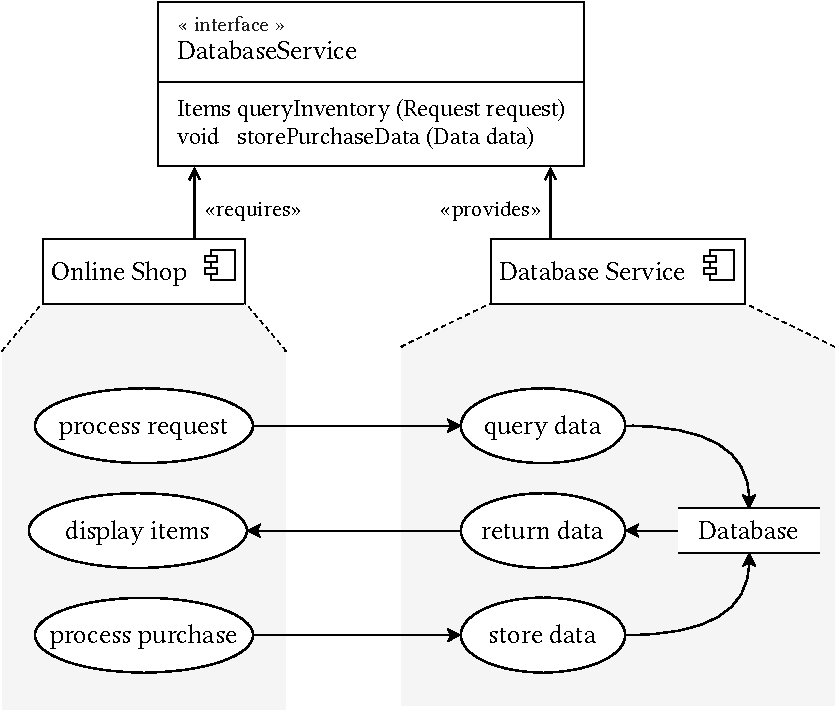
\includegraphics[width=0.8\linewidth]{figures/chapter6/mapping-example.pdf}
    \caption{Simplified mapping of the components of the running example to a \acf*{DFD}.}
    \label{fig:impactanalysis:representing:example}
\end{figure}

We start by explaining the relation of a high-level structural view like a \ac{PCM} component repository model and \acp{DFD} using our running example.
\autoref{fig:impactanalysis:representing:example} shows the simplified mapping of the two components \emph{Online Shop} and \emph{Database Service}, the interface that connects those components, and a \ac{DFD} showing the data flows of querying and purchasing items.
This mapping has been precisely defined by \textcite{seifermann_architectural_2022}, which includes the automated extraction of \acp{DFD} from the \ac{PCM}.

The components of \autoref{fig:impactanalysis:representing:example} are connected by an interface and additionally encapsulate their own behavior.
A \ac{PCM} component can have multiple intended purposes, e.g., the \emph{Online Shop} component is used to process item requests and to process purchases.
This is represented in the signatures of an interface and also becomes visible when looking at the \ac{DFD}.
Additionally, a single interface signature's behavior can be represented by multiple \ac{DFD} nodes, e.g., querying items with the signature \emph{queryInventory} involves the \emph{query data}, \emph{Database}, and \emph{return data} nodes.
Last, some information of the architectural model is not mapped to \acp{DFD}, e.g., every information related to the details of signatures and interfaces.
We find that there is no one-to-one mapping between an architectural model of the \ac{PCM} and a \ac{DFD}.
Both models can represent the same software system but show different concerns and abstraction levels.

When we discussed the difference of uncertainty \emph{sources} and the \emph{impact} of uncertainty on confidentiality, we stated that the locations can differ.
\autoref{fig:classification:example} showed an uncertainty source annotated to the customer using the \emph{Online Shop} and its potential impact to the \emph{Database Service}.
This relation also becomes visible in this mapping, illustrated in \autoref{fig:impactanalysis:representing:example}.
An uncertainty source in the input of the \emph{process request} node could affect the \emph{query data} node and transitively affect all other nodes in the flow, starting with the \emph{Database}.
Put simply, unspecified user input could lead to confidentiality violations in all of these nodes.
We find that a single uncertainty source can impact multiple nodes of a \ac{DFD} and that the representation of \acp{DFD} is suited to express this impact.

\begin{figure}
    \centering
    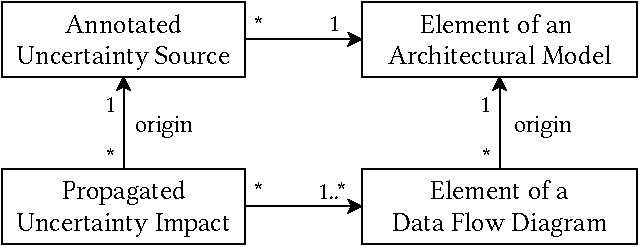
\includegraphics[width=0.65\linewidth]{figures/chapter6/relation-source-impact.pdf}
    \caption{Simplified view on the relation of software-architectural uncertainty sources, their propagated impact, software architectural models, and \acfp*{DFD}.}
    \label{fig:impactanalysis:representing:relation}
\end{figure}

These findings are summarized in \autoref{fig:impactanalysis:representing:relation}.
An element from the architectural model can be represented by zero, one, or many elements of \ac{DFD}.
Our example shows all three cases, as discussed previously.
When extracting \acp{DFD} from \ac{PCM} with the mapping of \textcite{seifermann_architectural_2022}, every \ac{DFD} element can be traced back to one originating element of the software architecture.

Software architects annotate identified uncertainty sources to the architectural model as this enables them to stay on the architectural abstraction \cite{hahner_architectural_2021}.
Although every uncertainty source is annotated to exactly one element of the software architecture, there is no limit how many uncertainty sources can be annotated to a single element.
Furthermore, there also can be elements without any annotated uncertainty, either because it has not yet been identified, or because it is currently not relevant.
See the procedure of uncertainty-aware analysis described in \autoref{sec:overview:procedure} for more details.

As shown in the discussion in \autoref{fig:impactanalysis:representing:example}, a single annotated uncertainty source can have multiple impact locations.
Similarly to the relation of architectural elements and \ac{DFD} elements, every impact can be traced back to one originating uncertainty source.
Put simply, once the confidentiality has been violated, software architects can trace the violation back to its cause, e.g., an overlooked uncertainty source.
A propagated uncertainty impact affects at least one \ac{DFD} element---or more, as seen in the running example.
Nevertheless, not every element of a \ac{DFD} has to be impacted by uncertainty.

This relation of uncertainty sources, their propagated impact, architectural models, and \acp{DFD} lays the foundation for all further discussions in this chapter.
Note that this is only one view on the relation of these concepts.
For instance, one could argue that a single uncertainty source can affect multiple elements of an architectural model\footnote{When I came back from SEAMS '23 in Australia where I presented this work, I had this very discussion with Shmuel Tyszberowicz. I conclude that allowing one uncertainty source to only affect a single element does not limit the generality as there could be infinite uncertainty sources that affect different elements and that are related and analyzed together.}.
For the sake of consistency, we are keeping this view for the remainder of this chapter. 

\finding{Architectural models are a suitable representation to be annotated with software-architectural uncertainty sources and \acfp{DFD} are suitable to represent their impact on confidentiality.
Multiple \ac{DFD} elements can represent a single element of the architectural model, and similarly, multiple elements of a \ac{DFD} can be impacted by a single uncertainty source.}


\subsection{A Meta Model of the Uncertainty Impact in Data Flow Diagrams}

In \autoref{sec:classification:classification}, we defined our classification of uncertainty that is tailored to confidentiality.
The category \emph{Architectural Element Type} is used as the primary category for annotating architectural models.
It offers five uncertainty types, i.e., five possible target elements of uncertainty.
Component uncertainty represents uncertainty in software components, connector uncertainty represents uncertainty in the wiring between components, interface uncertainty represents uncertainty in interfaces, external uncertainty represents uncertainty in resources, or users, and behavior uncertainty represents uncertainty in behavior descriptions.
See \autoref{table:classification:classification:architecturalelementtype} for details on the classification and \autoref{table:classification:mapping} for details on the relation of these options and \ac{DFD} elements.
We do not limit our modeling to a certain type of uncertainty, e.g., environmental uncertainty \cite{boltz_handling_2022}, or structural uncertainty \cite{walter_architectural_2022} in the following, but aim to support all five uncertainty types.

While these uncertainty types and their associated software-architectural elements are sufficient to document uncertainty sources, additional effort is required to also represent their impact, see \autoref{fig:impactanalysis:representing:relation}.
As discussed, confidentiality and the impact of uncertainty on confidentiality is best investigated using \acp{DFD}.
To this end, we extend the unified modeling primitives of \acp{DFD} \cite{seifermann_unified_2021}, which were introduced in \autoref{sec:foundations:dfd} and related to uncertainty in \autoref{sec:classification:dfd}.

\begin{figure}
    \centering
    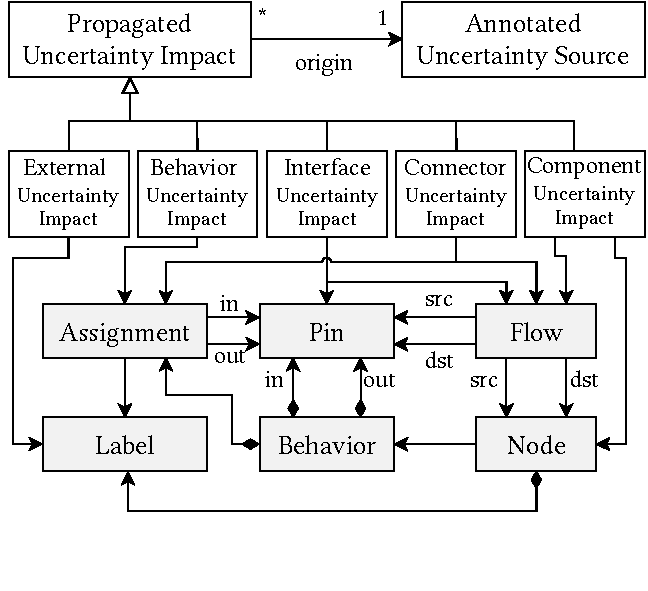
\includegraphics[width=0.7\linewidth]{figures/chapter6/metamodel-uia.pdf}
    \caption{Meta model of \acfp*{DFD} with the five different uncertainty impact types.}
    \label{fig:impactanalysis:representing:metamodel}
\end{figure}

\autoref{fig:impactanalysis:representing:metamodel} shows our meta model that combines the \ac{DFD} primitives (highlighted gray) and the five uncertainty types.
We extend the relation of uncertainty sources and their propagated impact to \ac{DFD} elements introduced in \autoref{fig:impactanalysis:representing:relation} based on the mapping shown in \autoref{table:classification:mapping}.
One \emph{Annotated Uncertainty Source} can have any number of \ac{DFD} elements affected by the \emph{Propagated Uncertainty Impact}.
We explain the relation of the five different uncertainty impact types and \ac{DFD} elements in the following.

\emph{Nodes} represent the system's structure and are affected by \emph{Component} uncertainty, e.g., Uncertainty \U{3} regarding the deployment of the \emph{Database Service} component in the running example would affect all nodes that represent this component.
We exemplified how to represent this in \acp{DAG} in \autoref{fig:classification:dag}.
\emph{Flows} connect these nodes by transmitting data and are affected by \emph{Connector Uncertainty}.
Additionally, \emph{Connector} uncertainty affects \emph{Assignments} of confidentiality-related labels, e.g., whether the user input is erroneous or malicious in Uncertainty \U{1} of the running example.
\emph{Flows} are also affected by \emph{Component} uncertainty, as altering components can change the flow of data, and also by \emph{Interface} uncertainty.
Primarily, \emph{Interface} uncertainty affects \emph{Pins} that decouple flows from a node and function as interfaces in the unified modeling primitives for \acp{DFD} \cite{seifermann_unified_2021}.
In \autoref{sec:classification:dfd}, we called these three uncertainty types \emph{secondary} uncertainty.
Also, in this meta model, we can see their broad impact on \ac{DFD} elements.
All \emph{secondary} uncertainty affects two different \ac{DFD} elements and can have a structural impact on the overall system.

In comparison, \emph{primary} uncertainty, i.e., \emph{Behavior} uncertainty and \emph{External} uncertainty, only affects one \ac{DFD} element.
Although this impact is more direct, we cannot make any claims on the severity or probability of confidentiality violations due to such uncertainty compared to \emph{secondary} uncertainty---this depends on the software system, the environment, and the uncertainty sources in both.
\emph{Behavior} uncertainty impacts the assignments that are used to represent the behavior of a \emph{Node}.
In our running example, Uncertainty \U{2} about the data processing could be represented as such an uncertainty source.
This would affect whether the behavior of the data processing node assigns the \emph{Labels} for validation or encryption.
Ultimately, this can lead to confidentiality violations similarly as all other uncertainty sources.
Last, \emph{Nodes} can also be described by \emph{Labels} to represent their confidentiality-related properties, which are affected by \emph{External} uncertainty.
In our running example, Uncertainty \U{4} can be represented as \emph{External} uncertainty affecting a label that expresses the trustworthiness of said \ac{DFD} node.

Our metamodel and its graphical representation in \autoref{fig:impactanalysis:representing:metamodel} demonstrate again the good fit of the five uncertainty types introduced by the category \emph{Architectural Element Type} of our classification to \acp{DFD}.
Every uncertainty impact affects another element type of the unified modeling primitives.
Additionally, all \emph{secondary} uncertainty types affect the flow, as discussed in \autoref{sec:classification:dfd}.
The only exception to this rule is the \emph{Behavior}, which has no associated uncertainty type because it only acts as a container for pins and assignments.
In sum, this meta model enables us to connect the uncertainty types from the software architecture to their corresponding impact type.
The representation based on \ac{DFD} elements simplifies the subsequent task of uncertainty propagation.

\finding{The propagated uncertainty impact can be represented by the five uncertainty types of the classification category \emph{Architectural Element Type}.
There is a direct relation of these types to the unified modeling primitives of \acfp{DFD}, which lays the foundation for the precise impact of uncertainty regarding confidentiality in software architectures.}


\subsection{Annotating Uncertainty Sources in the Palladio Component Model}

By now, we have discussed the relation of annotated uncertainty \emph{sources} and their propagated \emph{impact} with the more abstract view of architectural models and the more concrete view of \acp{DFD}.
However, to be applicable, one piece of the puzzle introduced in \autoref{fig:impactanalysis:representing:relation} is missing: The mapping of uncertainty sources to concrete elements of the architectural model.
Instead of only referring to architectural concepts like components, connectors, and interfaces, we discuss concrete annotation targets based on the \ac{ADL} \ac{PCM} \cite{reussner_modeling_2016} in the following.
These annotation targets can be derived by following the transformation \cite{seifermann_architectural_2022} from \ac{PCM} to \acp{DFD}.
Put simply, we investigate, which elements of the \ac{PCM} are relevant for \acp{DFD}---and thus, for confidentiality---and annotate uncertainty sources to them.
This not only concludes the relation discussed in this section but also lays the foundation for tool-supported modeling and automated analysis presented hereafter.

For the remainder of this chapter, we use the terminology known from the \ac{PCM}.
See \autoref{sec:foundations:architecture} for an overview of \ac{PCM}, or look into its comprehensive documentation \cite{reussner_modeling_2016,becker_palladio_2009,reussner_palladio_2011}.
To minimize confusion, we use the original terminology \cite{reussner_palladio_2011,reussner_modeling_2016} although there are slight deviations in the current Palladio implementation \cite{reussner_palladio_2024}.
However, this does only affect two \ac{PCM} element types used in the following: \emph{Signature} compared to \emph{OperationSignature}, and \emph{Interface} compared to \emph{OperationInterface}.
Note that there are also slight differences between the \ac{PCM} elements used for uncertainty impact analysis and those used to analyze confidentiality under uncertainty in later chapters because we only \emph{annotate} uncertainty source instead of altering the architectural model.
However, this is for purely pragmatic reasons that do not affect the underlying concepts.

\begin{table}
    \centering
    \begin{tabularx}{\linewidth}{lX}
        \toprule
        Uncertainty Type \,         & \ac{PCM} elements that can be annotated \\
        \midrule
        Component          & AssemblyContext \\
        Connector        & AssemblyConnector, ProvidedDelegationConnector \\
        Interface          & Signature, Interface \\
        External            & ResourceContainer, UsageScenario \\
        Behavior          & ExternalCallAction, EntryLevelSystemCall, SetVariableAction, BranchAction \\
        \bottomrule
    \end{tabularx}
    \caption{Mapping of the five uncertainty types to \acf*{PCM} elements.}%
    \label{table:impactanalysis:pcmmapping}
\end{table}

\autoref{table:impactanalysis:pcmmapping} shows the mapping of the uncertainty types to elements of the \ac{PCM} that can be annotated with this uncertainty source.
\emph{Component} uncertainty sources affect instances of components and are annotated to the \emph{AssemblyContext}.
\emph{AssemblyContexts} refer to component types from the \ac{PCM} component repository model and instantiate them within the concrete wiring of the \ac{PCM} system model.
Put simply, they represent concrete components and not component types and are thus suited to represent \emph{Component} uncertainty sources visible to software architects.
In our running example, we have two repository components, \emph{Online Shop} and \emph{Database Service}, which are both instantiated once.
To express uncertainty sources on type level, refer to \emph{Interface} uncertainty which annotates elements from the \ac{PCM} component repository model.

\emph{Connector} uncertainty affects inter-component structures, i.e., the wiring visible in the \ac{PCM} system model by using \emph{AssemblyConnectors}.
These connectors link concrete component instances, i.e., \emph{AssemblyContexts}, together.
In our running example, the connection of the \emph{Online Shop} and the \emph{Database Service} component is realized using such connectors.
Additionally, \emph{Connector} uncertainty can also affect \emph{ProvidedDelegationConnectors}.
These connectors represent system interfaces that can be used by users outside of the modeled system, e.g., in \emph{UsageScenarios}.
We support both connector types because both can be used to impact the usage of components, which is expressed by \emph{Connector} uncertainty.

\emph{Interface} uncertainty affects the interfaces that are defined in the \ac{PCM} component repository model.
Here, we support two levels of granularity: Either a single \emph{Signature} of an interface or the complete \emph{Interface}, i.e., all of its signatures, can be affected.
This enables software architects to minimize the annotation effort, e.g., to express that every communication over a selected interface is subject to uncertainty.
Note that in contrast to the first two uncertainty types, \emph{Interface} uncertainty is specified on a type level and not in the \ac{PCM} system model.
In our running example, the two components offer interfaces with multiple signatures.
One of these interfaces is illustrated in \autoref{fig:impactanalysis:representing:example}.

\emph{External} uncertainty affects the context of a software system, e.g., resources, and users.
It can be annotated to \emph{ResourceContainers}, which are part of the \ac{PCM} resource environment model, and \emph{UsageScenarios}, which are part of the \ac{PCM} usage model.
Both elements are part of the system environment and both can transitively affect the software system, e.g., because components are deployed to uncertainty-afflicted resources in the \ac{PCM} component allocation model.
Selecting these two elements to express environmental concerns that can affect confidentiality is inspired by architecture-based confidentiality analysis \cite{seifermann_data-driven_2019}.
In our running example, the \emph{On Premise Server} and the \emph{Cloud Service} represent \emph{ResourceContainers}.
The \emph{Customer} has multiple \emph{UsageScenarios}, e.g., browsing for items, or purchasing items.

\emph{Behavior} uncertainty affects the behavior of the software system and its users.
The behavior of the system is described in the form of \acfp{SEFF} in a \ac{PCM} component repository model.
Here, uncertainty can be annotated to \emph{ExternalCallActions} that represent components calling each other, \emph{SetVariableActions} that represent internal activities, and \emph{BranchActions} that can change the control flow.
All of these elements can affect the confidentiality of data flowing through them and are thus relevant for \emph{Behavior} uncertainty.
Last, \emph{Behavior} uncertainty can also be annotated in \emph{EntryLevelSystemCalls} that represent the user calling the system interface and are located in the \ac{PCM} usage model.
Although the location of classified uncertainty differs, i.e., uncertainty in the \emph{System Input} instead of the \emph{System Behavior}, the \emph{Architectural Element Type} option stays the same for impact analysis.
In our running example, the \emph{Customer} requesting the purchase of an item is represented by an \emph{EntryLevelSystemCall}, the storing of data called from the \emph{Online Shop} is realized with an \emph{ExternalCallAction}, and the data processing can be modeled with a \emph{SetVariableActions}.
For the sake of simplicity, we do not include branches.

In sum, all five types of uncertainty sources can be annotated to \ac{PCM} elements.
Based on the Palladio \cite{reussner_palladio_2024} tool support, existing modeling tools can be extended to support these annotations.
While uncertainty sources are best represented in the architectural model, their corresponding impact types are best represented in \acp{DFD}.
The uncertainty types of the category \emph{Architectural Element Type} originate from investigating existing classifications and \ac{DFD} notations.
Note that while these are generally applicable, alternative annotation targets other than the presented \ac{PCM} elements are possible \cite{benkler_architecture-based_2022}.
This is due to the nature of models representing reality, i.e., \ac{PCM} modeling software architecture \cite{stachowiak_allgemeine_1973}.

\finding{The source of the five uncertainty types of the category \emph{Architectural Element Type} can be annotated to the \acf{PCM}.
This \acf{ADL} can be extended to annotate uncertainty within the software system, e.g., its structure and behavior, and the system environment, e.g. usage scenarios and hardware resources.
Relating the five uncertainty types to concrete \ac{PCM} elements enables software architects to represent uncertainty sources on architectural abstraction.}





\section{Uncertainty Impact Analysis for Architectural Models}%
\label{sec:impactanalysis:pcmpropagation}

Building on the representation of uncertainty sources within architectural models, we can propagate the uncertainty to better understand its impact.
Starting from the annotation targets discussed in the previous section, we calculate this impact to define an \emph{uncertainty impact analysis} \cite{hezavehi_uncertainty_2021}.
Regarding confidentiality, this analysis requires two steps \cite{hahner_architecture-based_2023}.
First, the propagation within the architectural model, and second, the propagation in extracted \ac{DFD}.
As the uncertainty sources are annotated within the architectural model, we start with this part of the impact analysis.
As introduced previously, we will use the \ac{ADL} \ac{PCM} to detail the propagation rules.
This addresses Problem \PR{2}{2}.


\subsection{Adapting Change Impact Analysis to Uncertainty Propagation}

The name \enquote{uncertainty impact analysis} is inspired by architecture-based \emph{change impact analysis} \cite{heinrich_methodology_2018,rostami_architecture-based_2015,rostami_architecture-based_2017}.
Change impact analysis helps to predict the impact of changes in software architectures, e.g., changing interfaces, or replacing components \cite{rostami_architecture-based_2017}.
The early assessment and planning of change requests support software architects in software evolution.
The underlying concept of architecture-based change impact analysis is the propagation of changes in architectural models to identify potentially affected elements.
This requires the definition of propagation rules for each type of change, e.g., renaming a signature in an interface requires the providing component to also adapt its naming.

Regarding the \ac{PCM}, we build on \acf{KAMP} \cite{heinrich_methodology_2018,rostami_architecture-based_2015,rostami_architecture-based_2017,heinrich_architecture-based_2018,busch_architecture-based_2020}, as it provides a comprehensive foundation on change propagation.
It has been evaluated for many different use cases, e.g., architectural models \cite{rostami_architecture-based_2015}, business processes \cite{rostami_architecture-based_2017}, or automation systems \cite{heinrich_architecture-based_2018}.
\ac{KAMP} also supports the transitive propagation of changes, i.e., changes that occur due to other changes in the model, also called ripple effects \cite{bohner_software_2002}.
It has been used for other domain-spanning analyses \cite{heinrich_methodology_2018}, e.g., to define architecture-based attacker propagation \cite{walter_architectural_2022-1,walter_architecture-based_2023-1,walter_context-based_2023}.
Uncertainty is often also referred to as \emph{unanticipated change} \cite{hezavehi_uncertainty_2021,weyns_introduction_2020}.
Thus, it should not be surprising that the concept of change propagation can be reused%
\footnote{But in fact, it was. I have been trying to assess the impact of uncertainty on confidentiality for quite some time without making much progress. In 2021, after helping in an oral exam that covered the topic of change impact analysis, I asked myself: what if we could treat uncertainty like change in terms of its impact? Yes, we can, and the result is presented in this section. Call this serendipity if you want.}.

\finding{In architectural models, uncertainty can be treated like unanticipated changes.
This enables the leverage of propagation rules of architectural change impact analysis for the propagation of uncertainty.}

Change impact analysis defines three sets of elements \cite{busch_architecture-based_2020,bohner_software_2002}.
The \acf{SIS}, also sometimes called change set, contains the initial elements of the change request.
The \acf{AIS}, also sometimes called affected set, contains all elements that actually have to change due to the change request.
However, change impact analysis can only estimate this set \cite{busch_architecture-based_2020}.
The \acf{CIS}, also sometimes simply called impact set, represents this estimation.
Here, the goal of change impact analysis is to keep the estimation of the \ac{CIS} as close to the \ac{AIS} as possible.



\begin{table}
    \centering
    \begin{tabularx}{\linewidth}{llX}
        \toprule
        Uncertainty Source \,                   & Annotated \ac{PCM} element            & Exemplary name \\
        \midrule
        User input (\U{1})                & ProvidedDelegationConnector           & \emph{PurchaseInterface} \\
        Data processing (\U{2})           & SetVariableAction                     & \emph{processUserData} \\
        Component deployment (\U{3})      & AssemblyContext                       & \emph{DatabaseService} \\
        Provider trustworthiness (\U{4})  & ResourceContainer                     & \emph{CloudService} \\
        \bottomrule
    \end{tabularx}
    \caption{\acf*{SIS} representing the annotated uncertainty sources in the running example.}%
    \label{table:impactanalysis:sisexample}
\end{table}

We build on this terminology to apply these sets to \emph{uncertainty} impact analysis.
The \ac{SIS} represents the elements of the software architecture with annotated uncertainty sources.
Similarly to change impact analysis, this represents the starting point for any propagation.
Additionally, these elements are already affected by uncertainty, which could lead to confidentiality violations even without any further propagation.
In the running example, the \ac{SIS} contains the four elements from the software architecture that are annotated with the four uncertainty sources.
\autoref{table:impactanalysis:sisexample} shows the annotation of the uncertainty sources to the \ac{PCM} elements.
Note that these annotation targets only represent exemplary locations and could be modeled differently, see the discussion above.
We also include exemplary names comparable to those used in the running example model from our data set \cite{dataset}.

\begin{figure}
    \centering
    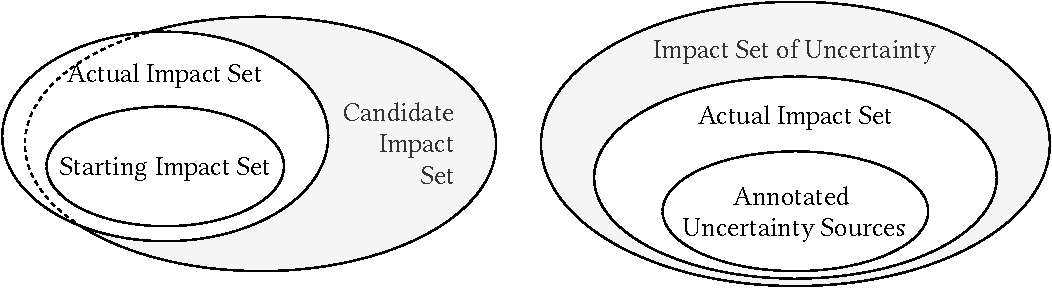
\includegraphics[width=\linewidth]{figures/chapter6/impactset.pdf}
    \caption{Informally illustrated relation of the different sets of change impact analysis (left) and uncertainty impact analysis (right).}
    \label{fig:impactanalysis:representing:sets}
\end{figure}

The \ac{AIS} represents the elements, that are actually impacted by the uncertainty sources in the \ac{SIS} and can violate confidentiality.
This set includes all elements from the \ac{SIS}, but can additionally contain elements that are directly or indirectly affected.
However, we can only estimate this set.
Similarly to change impact analysis, an uncertainty impact analysis yields a \ac{CIS}, which represents an estimation of potentially impacted elements.
Here, we require a more strict relation. 
While change impact analysis may underestimate the \ac{CIS} compared to the \ac{AIS}, uncertainty impact analysis regarding confidentiality shall always overestimate the \ac{CIS}.
Put simply, an ignored impact of uncertainty could lead to overlooked confidentiality violations.
Especially regarding security-related quality properties like confidentiality, high recall can be more important than high precision \cite{hahner_architecture-based_2023}.
Additionally, the uncertainty impact analysis is used for an \emph{early} prediction and assessment of uncertainty, not for precise analysis, see \autoref{sec:overview:procedure}.
This has to be considered in defining the propagation rules for uncertainty.
For the sake of simplicity, we refer to the \ac{AIS} as the actual impact set and to the \ac{CIS} simply as \emph{impact set} of uncertainty.
The relation of the terminology of both analyses is illustrated in \autoref{fig:impactanalysis:representing:sets}.

In the following, we describe propagation rules for all annotation targets of uncertainty sources in the \ac{PCM}.
They have to be described separately for each relevant \ac{PCM} element as they are specific to the \ac{ADL} \ac{PCM}.
Nevertheless, the general concept of architectural uncertainty propagation is generalizable \cite{camara_uncertainty_2024}.
The goal of uncertainty propagation in the architectural model is to identify all uncertainty-afflicted elements of the software architecture, which are later represented by the extracted \ac{DFD} \cite{seifermann_architectural_2022}.
In most cases, this means starting with propagation rules from change impact analysis and then identifying relevant \ac{SEFF} actions, as these are relevant to the \ac{DFD} extraction of \textcite{seifermann_architectural_2022}.
This step is important because of the abstraction gap between the representations of \acp{DFD} and the \ac{PCM}, see \autoref{sec:impactanalysis:representing}.
By identifying those elements, the coupling of the architectural impact analysis with the propagation of uncertainty in \acp{DFD} is simplified.
Only propagating uncertainty in \acp{DFD} is not sufficient due to the missing information compared to architectural models.

\finding{Uncertainty impact analysis regarding confidentiality in architectural models consists of two steps.
First, identifying directly and indirectly affected elements, following the propagation rules of change impact analysis.
Second, identifying originating elements of the transformation to \acp{DFD}, which are relevant for further propagation.}


\subsection{Uncertainty Propagation of Component Uncertainty}

\emph{Component} uncertainty can only be annotated to \emph{AssemblyContexts}, which simplifies the propagation logic.
\autoref{alg:impactanalysis:component} shows the propagation algorithm.
Every propagation algorithm is called with the annotated uncertainty source contained in the parameter \emph{uncertainty} and the \ac{PCM} model contained in the parameter \emph{model}.
We always start by creating an empty list of results and retrieving the model element that has been annotated with the uncertainty source, following the relation specified in \autoref{fig:impactanalysis:representing:relation}.

\begin{algorithm}
    \caption{Algorithm for component uncertainty propagation}
    \label{alg:impactanalysis:component}
    \begin{algorithmic}[1]
        \Procedure{\function{propagateComponentUncertainty}}{$\var{uncertainty}, \var{model}$}
            \algindentskip
            \State $\var{result} \gets \emptyset$
            \State $\var{assemblyContext} \gets \function{getAnnotatedElement}(\var{uncertainty}, \var{model})$
            \State $\var{component} \gets \function{getRepositoryComponent}(\var{assemblyContext}, \var{model})$ \label{alg:impactanalysis:component:4}
            \State $\var{seffs} \gets \function{getSEFFs}(\var{component}, \var{model})$ \label{alg:impactanalysis:component:5}
            \algblockskip

            \For{$\var{seff} \in \var{seffs}$} \label{alg:impactanalysis:component:6} \Comment{Component uncertainty affects all SEFFs of a component}
                \State $\var{startAction} \gets \function{retrieveStartAction}(\var{seff}, \var{model})$
                \State $\var{result} \gets \var{result} \cup \setted{\var{startAction}}$ \label{alg:impactanalysis:component:11}
            \EndFor
            \algblockskip
        
            \State \Return{$\function{applyToAssembly}(\var{result},\var{assemblyContext})$} \label{alg:impactanalysis:component:10}
            \algindentskip
        \EndProcedure   
    \end{algorithmic}
\end{algorithm}

In the case of \emph{AssemblyContexts}, which represent instantiated components, we retrieve the component type from the \ac{PCM} component repository model in \autoref{alg:impactanalysis:component:4} and then query for its \acp{SEFF} in \autoref{alg:impactanalysis:component:5}.
A component provides one \ac{SEFF} for each signature of a provided interface.
For instance, in our running example, the \emph{Database Service} provides \acp{SEFF} for the operations \emph{queryInventory} and \emph{storePurchaseData}, see \autoref{fig:impactanalysis:representing:example}.

\begin{algorithm}
    \caption{Algorithm for retrieving the initial StartAction of a \ac*{SEFF}}
    \label{alg:impactanalysis:helperseff}
    \begin{algorithmic}[1]
        \Procedure{\function{retrieveStartAction}}{$\var{seff}, \var{model}$}
            \algindentskip
            \State $\var{actions} \gets \function{getActions}(\var{seff}, \var{model})$
            \For{$\var{action} \in \var{actions}$}
                \If{$\function{typeOf}(\var{action}) = \datatype{StartAction}$} \label{alg:impactanalysis:helperseff:4}
                    \State $\var{startAction} \gets \var{action}$ \Comment{The first start action is the start of the SEFF}
                    \State \Return{$\var{startAction}$}
                \EndIf
            \EndFor
            \algindentskip
        \EndProcedure   
    \end{algorithmic}
\end{algorithm}

From the perspective of the change impact analysis, these \acp{SEFF} are impacted by a change to the component.
To close the gap to the representation in \acp{DFD}, we need to retrieve the initial actions of all \acp{SEFF} that are represented as \ac{DFD} nodes \cite{seifermann_architectural_2022}.
We show this separately in \autoref{alg:impactanalysis:helperseff} because we reuse this functionality several times in other algorithms.
A \ac{SEFF} contains actions that represent its behavior, comparable to \ac{UML} activity diagrams.
The initial actions have the \ac{PCM} element type \emph{StartAction}, see \autoref{alg:impactanalysis:helperseff:4}.
Using the functionality described in \autoref{alg:impactanalysis:helperseff}, we iterate over all \acp{SEFF}, starting in \autoref{alg:impactanalysis:component:6}.
Once we found this action, we add it to the results list in \autoref{alg:impactanalysis:component:11}.
The algorithm ends after all initial \emph{StartActions} of all \acp{SEFF} have been identified and returns the result.

Note that we skip some Palladio \cite{reussner_palladio_2024} implementation details.
First, we do not show required type casts, e.g., from \emph{RepositoryComponent} to \emph{BasicComponent} to retrieve the \acp{SEFF}.
Second, we hide method calls, e.g., to retrieve all actions, a detour from the \ac{SEFF} through its behavior is required.
Third, we skip the handling of the system context.
This step is required because \acp{SEFF} are defined in the \ac{PCM} component repository model and could be instantiated in multiple assemblies.
However, we are only interested in those actions representing the \emph{AssemblyContext} that is annotated with the component uncertainty.
We illustrate this with a method call of \emph{applyToAssembly} in \autoref{alg:impactanalysis:component:10}.
Last, we assume well-formed \ac{PCM} models without errors.
All of these details would only greatly increase the size of the algorithms without contributing to their understandability.
To see the detailed implementation of all algorithms, please look into the data set \cite{dataset}.


\subsection{Uncertainty Propagation of Interface Uncertainty}

\emph{Interface} uncertainty can be annotated to full interfaces or selected signatures.
Uncertainty affecting interfaces results in a wide impact due to their central role in software systems.
The propagation of interface uncertainty requires the most extensive algorithm.
We split the propagation into three parts.
First, we identify all components and their actions that implement the interface in \autoref{alg:impactanalysis:interface:startaction}.
Second, we identify all actions that represent calls to the interface in \autoref{alg:impactanalysis:interface:externalcallaction}.
Third, we identify all system calls from \emph{UsageScenarios} to the interface in \autoref{alg:impactanalysis:interface:entrylevelsystemcall}.
These three steps are required as we cannot make any assumptions on the usage of the interface, e.g., to wire components or to represent a user interface.
By combining these three steps, we specify the algorithm for interface uncertainty propagation in \autoref{alg:impactanalysis:interface}.

\emph{Interface} uncertainty affects the \ac{PCM} component repository model and is not limited single assemblies like \emph{Component} uncertainty.
Thus, the impact set can be even bigger, as all \emph{AssemblyContexts} of a component can be affected.
Put simply, if a component that is used multiple times in a software system has uncertainty in its interface, it affects all instances of this component and also all components that depend on these instances.

\begin{algorithm}
    \caption{Algorithm for retrieving all StartActions that describe a signature}
    \label{alg:impactanalysis:interface:startaction}
    \begin{algorithmic}[1]
        \Procedure{\function{retrieveStartActionsBySignature}}{$\var{signature}, \var{model}$}
            \algindentskip
            \State $\var{result} \gets \emptyset$
            \State $\var{allComponents} \gets \function{getAllRepositoryComponents}(\var{model})$
            \algblockskip

            \For{$\var{component} \in allComponents$}
                \State $\var{seffs} \gets \function{getSEFFs}(\var{component}, \var{model})$
                \For{$\var{seff} \in \var{seffs}$} \Comment{Find called StartActions}
                    \If{$\function{getDescribedSignature}(\var{seff}, \var{model}) = signature$} \label{alg:impactanalysis:interface:startaction:7}
                        \State $\var{startAction} \gets \function{retrieveStartAction}(\var{seff}, \var{model})$ \label{alg:impactanalysis:interface:startaction:8}
                        \State $\var{result} \gets \var{result} \cup \setted{\var{startAction}}$
                    \EndIf
                \EndFor
            \EndFor
            \algblockskip

            \State \Return{$\var{result}$}
            \algindentskip
        \EndProcedure   
    \end{algorithmic}
\end{algorithm}

\autoref{alg:impactanalysis:interface:startaction} shows the algorithm to identify all \acp{SEFF} that implement a signature of an interface.
Regarding change impact analysis, this resembles the adaption of all implementations of an interface, e.g., due to a rename of a signature.
We iterate over all \acp{SEFF} of all components in the \ac{PCM} component repository model to find matching \emph{StartActions}.
The retrieval logic is similar to \emph{Component} uncertainty with two important distinctions.
First, the retrieval is not limited to a single \emph{AssemblyContext} but includes all components.
Second, the algorithm only considers \acp{SEFF} that implement the given signature of the interface.
Not necessarily all \acp{SEFF} of a component have to implement an interface because components can also provide multiple interfaces.
This filter is realized in \autoref{alg:impactanalysis:interface:startaction:7}.
Afterward, we retrieve the \emph{StartAction} in \autoref{alg:impactanalysis:interface:startaction:8} using the logic described with \autoref{alg:impactanalysis:helperseff}.
In our running example, retrieving the \emph{StartAction} of the \ac{SEFF} that implements the signature \emph{queryInventory} would yield a \emph{StartAction} of the component \emph{Database Service} because this component provides the interface that contains the signature, see \autoref{fig:impactanalysis:representing:example}.

\begin{algorithm}
    \caption{Algorithm for retrieving all ExternalCallActions that call a signature}
    \label{alg:impactanalysis:interface:externalcallaction}
    \begin{algorithmic}[1]
        \Procedure{\function{retrieveExternalCallsToSignature}}{$\var{signature}, \var{model}$}
            \algindentskip
            \State $\var{result} \gets \emptyset$
            \State $\var{allComponents} \gets \function{getAllRepositoryComponents}(\var{model})$
            \algblockskip

            \For{$\var{component} \in allComponents$} \Comment{Iterate over all available actions} \label{alg:impactanalysis:interface:externalcallaction:4}
                \State $\var{seffs} \gets \function{getSEFFs}(\var{component}, \var{model})$
                \For{$\var{seff} \in \var{seffs}$} 
                    \State $\var{actions} \gets \function{getActions}(\var{seff}, \var{model})$
                    \For{$\var{action} \in \var{actions}$} \Comment{Find calling ExternalCallActions}
                        \If{$\function{typeOf}(\var{action}) = \datatype{ExternalCallAction}$} 
                            \If{$\function{getCalledSignature}(\var{action}, \var{model}) = signature$} \label{alg:impactanalysis:interface:externalcallaction:10}
                                \State $\var{result} \gets \var{result} \cup \setted{\var{action}}$
                            \EndIf
                        \EndIf
                    \EndFor
                \EndFor
            \EndFor
            \algblockskip

            \State \Return{$\var{result}$}
            \algindentskip
        \EndProcedure   
    \end{algorithmic}
\end{algorithm}

\autoref{alg:impactanalysis:interface:externalcallaction} shows the algorithm to identify all system actions that call a signature of an interface.
In the \ac{PCM}, calls between components are modeled in \ac{SEFF} using \emph{ExternalCallActions} \cite{becker_palladio_2009}.
Regarding change impact analysis, this resembles adapting the call to an interface after the interface has changed.
To identify the impacted \emph{ExternalCallActions}, we have to iterate over all available actions starting in \autoref{alg:impactanalysis:interface:externalcallaction:4}.
This is achieved by iterating over all components, all of its \acp{SEFF} and over all of their actions.
If the action represents an \emph{ExternalCallAction}, we check its called signature in \autoref{alg:impactanalysis:interface:externalcallaction:10}.
All actions that fit these conditions are added to the result.
These would also be part of the \ac{CIS} of the change impact analysis \ac{KAMP} \cite{busch_architecture-based_2020}.
In our running example detailed in \autoref{fig:impactanalysis:representing:example}, an \emph{ExternalCallAction} is used after the processing of the purchase in the \emph{Online Shop} to initiate the storing of the data in the \emph{Database Service}.
To minimize costly iterations, concrete implementations of this algorithm can cache identified \emph{ExternalCallActions} or use other query methods, which return all occurrences of an element type within a model \cite{dataset}---we show the generic approach of iterating over all components to keep the algorithm as simple as possible.


\begin{algorithm}
    \caption{Algorithm for retrieving all EntryLevelSystemCalls that call a signature}
    \label{alg:impactanalysis:interface:entrylevelsystemcall}
    \begin{algorithmic}[1]
        \Procedure{\function{retrieveEntryCallsToSignature}}{$\var{signature}, \var{model}$}
        \algindentskip
        \State $\var{result} \gets \emptyset$
        \State $\var{allUsageScenarios} \gets \function{getAllUsageScenarios}(\var{model})$
        \algblockskip

        \For{$\var{usageScenario} \in allUsageScenarios$} \label{alg:impactanalysis:interface:entrylevelsystemcall:4}
            \State $\var{actions} \gets \function{getActions}(\var{usageScenario}, \var{model})$
            \For{$\var{action} \in \var{actions}$} \Comment{Find calling EntryLevelSystemCalls}
                \If{$\function{typeOf}(\var{action}) = \datatype{EntryLevelSystemCall}$} \label{alg:impactanalysis:interface:entrylevelsystemcall:7}
                    \If{$\function{getCalledSignature}(\var{action}, \var{model}) = signature$} \label{alg:impactanalysis:interface:entrylevelsystemcall:8}
                        \State $\var{result} \gets \var{result} \cup \setted{\var{action}}$
                    \EndIf
                \EndIf
            \EndFor
        \EndFor
        \algblockskip

        \State \Return{$\var{result}$}
        \algindentskip
        \EndProcedure   
    \end{algorithmic}
\end{algorithm}

\autoref{alg:impactanalysis:interface:entrylevelsystemcall} shows the algorithm to identify all calls from a \emph{UsageScenario} to a signature of an interface.
In the \ac{PCM}, calls to the the system are modeled using \emph{EntryLevelSystemCalls}.
As discussed above, this step is required as we cannot assume that an interface is only used between components.
This step is also performed by change impact analysis \cite{busch_architecture-based_2020}.
To identify relevant \emph{EntryLevelSystemCalls}, we iterate over all actions of all \emph{UsageScenarios}, starting in \autoref{alg:impactanalysis:interface:entrylevelsystemcall:4}.
We first check for the type of the action in \autoref{alg:impactanalysis:interface:entrylevelsystemcall:7}, and if it represents an \emph{EntryLevelSystemCall}, we check the called signature in \autoref{alg:impactanalysis:interface:entrylevelsystemcall:8}.
Afterward, the actions are added to the result.
This procedure closely resembles the retrieval of impacted \emph{ExternalCallActions}.
Here, the main difference is that we do not analyze the behavior of a component but the user behavior that is modeled in the \ac{PCM} usage model.
In our running example, all calls of the \emph{Customer} to the \emph{Online Shop} are modeled using \emph{EntryLevelSystemCalls}, e.g., the querying of items.


\begin{algorithm}
    \caption{Algorithm for interface uncertainty propagation}
    \label{alg:impactanalysis:interface}
    \begin{algorithmic}[1]
        \Procedure{\function{propagateInterfaceUncertainty}}{$\var{uncertainty}, \var{model}$}
        \algindentskip
        \State $\var{result} \gets \emptyset$
        \State $\var{affectedSignatures} \gets \emptyset$
        \State $\var{annotatedElement} \gets \function{getAnnotatedElement}(\var{uncertainty}, \var{model})$ \label{alg:impactanalysis:interface:4}
        \algblockskip

        \Switch{$\function{typeOf}(\var{annotatedElement})$} \label{alg:impactanalysis:interface:5}
            \Case{$\datatype{Signature}$}
                \State $\var{affectedSignatures} \gets \setted{\var{annotatedElement}}$
            \EndCase
            \Case{$\datatype{Interface}$} \Comment{Decompose the interface}
                \State $\var{affectedSignatures} \gets \function{getSignatures}(\var{annotatedElement}, \var{model})$
            \EndCase
        \EndSwitch
        \algblockskip

        \For{$\var{signature} \in \var{affectedSignatures}$} \Comment{Combine the three retrieval steps} \label{alg:impactanalysis:interface:10}
            \State $\var{result} \gets \var{result} \cup \function{retrieveStartActionsBySignature}(\var{signature}, \var{model})$
            \State $\var{result} \gets \var{result} \cup \function{retrieveExternalCallsToSignature}(\var{signature}, \var{model})$
            \State $\var{result} \gets \var{result} \cup \function{retrieveEntryCallsToSignature}(\var{signature}, \var{model})$
        \EndFor
        \algblockskip

        \State \Return{$\var{result}$}
        \algindentskip
        \EndProcedure   
    \end{algorithmic}
\end{algorithm}

We combine the algorithms \ref{alg:impactanalysis:interface:startaction}, \ref{alg:impactanalysis:interface:externalcallaction}, and \ref{alg:impactanalysis:interface:entrylevelsystemcall} to specify the propagation algorithm for \emph{Interface} uncertainty in \autoref{alg:impactanalysis:interface}.
After retrieving the element that has been annotated with uncertainty in \autoref{alg:impactanalysis:interface:4}, we perform a type check in \autoref{alg:impactanalysis:interface:5}.
If the annotated element is an \emph{Interface}, we decompose the interface into its signatures and add it to the list of affected signatures.
If the annotated element is a \emph{Signature}, this list only consists of this single signature.
This resembles one propagation step from change impact analysis \cite{rostami_architecture-based_2017,busch_architecture-based_2020} and enables the treatment of both annotations targets similarly in the following.
Put simply, annotating a signature instead of an interface increases the precision of the result but only has a negligible effect on the propagation logic.
Afterward, we iterate over all signatures in \autoref{alg:impactanalysis:interface:10}.
For each signature, we perform the three retrieval tasks, i.e., retrieving affected \emph{StartActions}, \emph{ExternalCallActions}, and \emph{EntryLevelSystemCalls}.
The combined result is returned from the algorithm.
Note that this does not cause any typing problems, as we expect \emph{any} action as a result, similarly to all other propagation algorithms.

In our running example, an \emph{Interface} uncertainty that has been annotated to the interface between the \emph{Online Shop} and the \emph{Database Service} components would yield affected elements from both components.
This includes \emph{StartActions} from \acp{SEFF} of all implementations of operations specified in the interface and also \emph{ExternalCallActions} to these operations.
However, as this interface is only used between components, no \emph{EntryLevelSystemCalls} would be directly affected.
Note that there is no call to \emph{applyToAssembly} as we do not limit the impact of uncertainty to a single assembly.
For instance, if the \emph{Database Service} component would be used in multiple locations in the system, all instances would be affected by the uncertainty.

Similarly to the propagation of \emph{Component} uncertainty shown in \autoref{alg:impactanalysis:component}, we hide implementation details.
This includes chained method calls, e.g., to retrieve all actions of a \emph{UsageScenario}, a detour over its behavior is required \cite{reussner_palladio_2024}.
Although all algorithms presented in this section contain several loops, we do not expect problems regarding their scalability in practice.
First, the sets to iterate over are usually small, e.g., because a properly defined interface only contains a small number of signatures \cite{martin_clean_2017}.
Second, there are many ways to speed up the implementation, e.g., by using caches, or by integrating the extracted \acp{DFD} early in the propagation to filter potential candidates.
We apply many of these optimizations in our implementation that are available in the data set \cite{dataset}.


\subsection{Uncertainty Propagation of Connector Uncertainty}

\begin{algorithm}
    \caption{Algorithm for connector uncertainty propagation}
    \label{alg:impactanalysis:connector}
    \begin{algorithmic}[1]
        \Procedure{\function{propagateConnectorUncertainty}}{$\var{uncertainty}, \var{model}$}
            \algindentskip
            \State $\var{result} \gets \emptyset$
            \State $\var{connector} \gets \function{getAnnotatedElement}(\var{uncertainty}, \var{model})$
            \State $\var{interface} \gets \function{getInterface}(\var{connector}, \var{model})$ \label{alg:impactanalysis:connector:4}
            \State $\var{signatures} \gets \function{getSignatures}(\var{interface}, \var{model})$
            \State $\var{calledAssembly} \gets \function{getProvidingAssemblyContext}(\var{connector}, \var{model})$ \label{alg:impactanalysis:connector:6}
            \algblockskip

            \For{$\var{signature} \in \var{signatures}$}  \Comment{Find called StartActions} \label{alg:impactanalysis:connector:7}
                \State $\var{actions} \gets \function{retrieveStartActionsBySignature}(\var{signature}, \var{model})$
                \State $\var{result} \gets \var{result} \cup \function{applyToAssembly}(\var{actions},\var{calledAssembly})$ \label{alg:impactanalysis:connector:9}
            \EndFor
            \algblockskip

            \Switch{$\function{typeOf}(\var{connector})$} \label{alg:impactanalysis:connector:11}
                \Case{$\datatype{AssemblyConnector}$}
                    \State $\var{callingAssembly} \gets \function{getRequiringAssemblyContext}(\var{connector}, \var{model})$ \label{alg:impactanalysis:connector:13}
                    \algblockskip
                    \For{$\var{signature} \in \var{signatures}$}  \Comment{Find calling ExternalCallActions} \label{alg:impactanalysis:connector:14}
                        \State $\var{actions} \gets \function{retrieveExternalCallsToSignature}(\var{signature}, \var{model})$
                        \State $\var{result} \gets \var{result} \cup \function{applyToAssembly}(\var{actions},\var{callingAssembly})$ \label{alg:impactanalysis:connector:16}
                    \EndFor
                    \algblockskip
                \EndCase
                \Case{$\datatype{ProvidedDelegationConnector}$} 
                    \State $\var{delegatedContext} \gets \function{getDelegatedContext}(\var{connector}, \var{model})$ \label{alg:impactanalysis:connector:19}
                    \algblockskip
                    \For{$\var{signature} \in \var{signatures}$}  \Comment{Find calling EntryLevelSystemCalls} \label{alg:impactanalysis:connector:20}
                        \State $\var{actions} \gets \function{retrieveEntryCallsToSignature}(\var{signature}, \var{model})$
                        \State $\var{result} \gets \var{result} \cup \function{applyToAssembly}(\var{actions},\var{delegatedContext})$ \label{alg:impactanalysis:connector:22}
                    \EndFor
                    \algblockskip
                \EndCase
            \EndSwitch
            \algblockskip

            \State \Return{$\var{result}$}
            \algindentskip
        \EndProcedure   
    \end{algorithmic}
\end{algorithm}

\emph{Connector} uncertainty can be annotated to \emph{AssemblyConnectors} and \emph{ProvidedDelegationConnectors}.
\autoref{alg:impactanalysis:connector} shows the propagation algorithm.
Uncertainty affecting connectors behaves comparable to \emph{Interface} uncertainty.
It impacts both the called component and the calling entity, which can be another component or a user.
The main difference is that connectors are specific to assemblies and modeled in the \ac{PCM} system model.
We can reuse the logic defined for \emph{Interface} uncertainty hereabove but we have to relate the results to the correct \emph{AssemblyContexts}.

A \emph{Connector} represents the wiring of two entities within a software system, expressed, e.g., using the ball and socket notation of \ac{UML} component diagrams as shown in \autoref{fig:runningexample:architecture}.
All connectors are based on an interface that we retrieve in \autoref{alg:impactanalysis:connector:4}.
In the \ac{PCM}, we support \emph{AssemblyConnectors} between two components and \emph{ProvidedDelegationConnectors} that can be referred to outside the system in \emph{UsageScenarios}.

Independent of its type, a connector always has a providing \emph{AssemblyContext}, representing the component that implements the provided interface.
This called \emph{AssemblyContext} is retrieved in \autoref{alg:impactanalysis:connector:6}.
Afterward, we find all called \emph{StartActions} beginning in \autoref{alg:impactanalysis:connector:7}.
Here, we can reuse the logic defined for \emph{Interface} uncertainty in \autoref{alg:impactanalysis:interface:startaction}.
The only difference is that we are only interested in those \emph{StartActions} that represent the connected \emph{AssemblyContext}.
This is realized in \autoref{alg:impactanalysis:connector:9}, similarly to \emph{Component} uncertainty.

Afterward, we address the calling side, starting in \autoref{alg:impactanalysis:connector:11}.
In the case of an \emph{AssemblyConnector}, we retrieve the calling assembly that requires the interface represented by the connector in \autoref{alg:impactanalysis:connector:13}.
We use the logic defined for \emph{Interface} uncertainty in \autoref{alg:impactanalysis:interface:externalcallaction} to find the according \emph{ExternalCallActions} in \autoref{alg:impactanalysis:connector:14}.
Again, we have to apply the correct \emph{AssemblyContext}.
This time, this is achieved using the calling assembly in \autoref{alg:impactanalysis:connector:16}.
In the case of a \emph{ProvidedDelegationConnector}, we proceed with the retrieval of \emph{EntryLevelSystemCalls}.
Here, we are only interested in the provided delegation of the system interface, which is retrieved in \autoref{alg:impactanalysis:connector:19}.
After receiving candidate \emph{ExternalCallActions} in \autoref{alg:impactanalysis:connector:20}, we apply again the correct context in \autoref{alg:impactanalysis:connector:22}.

Put simply, to propagate \emph{Connector} uncertainty we proceed as if the interface that is represented would be affected by \emph{Interface} uncertainty.
Every potentially impacted action is then applied to the correct \emph{AssemblyContext}, either called or calling.
Regarding change impact analysis, this resembles the required changes both in the component that implements an interface and the component requiring an interface.
Besides the handling of \emph{AssemblyContexts} and indirection from the \emph{Connector} to interfaces, another difference is the distinction of the connector type.
When propagating \emph{Interface} uncertainty, we only use the \ac{PCM} component repository model and we cannot make assumptions on the interface use, i.e., whether the interface is only used between components or also in \emph{UsageScenarios}.
Opposite to this, \emph{Connectors} are part of the \ac{PCM} system model that models this information.
Thus, we are not required to handle all cases and can either retrieve \emph{ExternalCallActions} or \emph{EntryLevelSystemCalls}, but not both.
In our running example, the results of an \emph{Interface} uncertainty and a \emph{Connector} uncertainty annotated between the \emph{Online Shop} and \emph{Database Service} components are identical because both components are only referred by a single \emph{AssemblyContext}.
Similarly to the other algorithms, we simplified some chained method calls and we refer to the data set for more details \cite{dataset}.


\subsection{Uncertainty Propagation of External Uncertainty}

\begin{algorithm}
    \caption{Algorithm for external uncertainty propagation}
    \label{alg:impactanalysis:external}
    \begin{algorithmic}[1]
        \Procedure{\function{propagateExternalUncertainty}}{$\var{uncertainty}, \var{model}$}
        \algindentskip
        \State $\var{result} \gets \emptyset$
        \State $\var{annotatedElement} \gets \function{getAnnotatedElement}(\var{uncertainty}, \var{model})$
        \algblockskip

        \Switch{$\function{typeOf}(\var{annotatedElement})$} \label{alg:impactanalysis:external:4}
            \Case{$\datatype{UsageScenario}$}
                \State $\var{actions} \gets \function{getActions}(\var{annotatedElement}, \var{model})$ \label{alg:impactanalysis:external:6}
                \For{$\var{action} \in \var{actions}$} \Comment{Find all EntryLevelSystemCalls}
                    \If{$\function{typeOf}(\var{action}) = \datatype{EntryLevelSystemCall}$}
                        \State $\var{result} \gets \var{result} \cup \setted{\var{action}}$
                    \EndIf
                \EndFor
                \algblockskip
            \EndCase
            \Case{$\datatype{ResourceContainer}$} 
                \State $\var{allAssemblyContexts} \gets \function{getAllAssemblyContexts}(\var{model})$ \label{alg:impactanalysis:external:13}
                \For{$\var{context} \in \var{allAssemblyContexts}$} \Comment{Find all actions}
                    \If{$\function{getAllocation}(\var{context}, \var{model}) = annotatedElement$} \label{alg:impactanalysis:external:15}
                        \State $\var{component} \gets \function{getRepositoryComponent}(\var{context}, \var{model})$
                        \State $\var{seffs} \gets \function{getSEFFs}(\var{component}, \var{model})$
                        \For{$\var{seff} \in \var{seffs}$}
                            \State $\var{actions} \gets \function{getActions}(\var{seff}, \var{model})$ 
                            \State $\var{result} \gets \var{result} \cup \function{applyToAssembly}(\var{actions},\var{context})$ \label{alg:impactanalysis:external:20}
                        \EndFor
                    \EndIf
                \EndFor
            \EndCase
        \EndSwitch
        \algblockskip
        \State \Return{$\var{result}$}
        \algindentskip
        \EndProcedure   
    \end{algorithmic}
\end{algorithm}

\emph{External} uncertainty can be annotated to \emph{ResourceContainers} and \emph{UsageScenarios}.
\autoref{alg:impactanalysis:external} shows the propagation algorithm.
\emph{ResourceContainers} are part of the \ac{PCM} resource environment model and \emph{UsageScenarios} are part of the \ac{PCM} usage model.
Although the propagation logic differs, it states the same: Find all actions that belong to the element that has been annotated with \emph{external} uncertainty.
Put simply, if a resource container or a user is affected by uncertainty, we cannot trust any of their actions.

The algorithm starts with a large switch statement in \autoref{alg:impactanalysis:external:4}.
In the case of an annotated \emph{UsageScenario}, we iterate over all of its actions, starting in \autoref{alg:impactanalysis:external:6}.
This is similar to the identification of relevant \emph{EntryLevelSystemCalls} of \emph{Interface} or \emph{Connector} uncertainty.
The major difference is that we do not filter for a specific signature, but add all identified \emph{EntryLevelSystemCalls}, as they could all be affected by uncertainty.
We only consider \emph{EntryLevelSystemCalls} as they represent the only user actions that are considered in the extraction of \acp{DFD} \cite{seifermann_architectural_2022}.

In the case of an annotated \emph{ResourceContainer}, we have to identify all \emph{AssemblyContexts} that are allocated on this container.
We retrieve all \emph{AssemblyContexts} from the \ac{PCM} system model in \autoref{alg:impactanalysis:external:13} and iterate over them.
For each assembly, we check its allocation using the \ac{PCM} allocation model in \autoref{alg:impactanalysis:external:15}.
If an \emph{AssemblyContext} is deployed on the \emph{ResourceContainer} that has been annotated with the uncertainty, we add all of its actions to the result list in \autoref{alg:impactanalysis:external:20}.
This step is comparable to the propagation of \emph{Component} uncertainty.
However, we do not limit the propagation to \emph{StartActions} as every action could be affected by uncertainty.

In the running example, an \emph{external} uncertainty annotated to the \emph{ResourceContainer} where the \emph{Online Shop} gets deployed would affect all of its actions.
In the simplified illustration shown in \autoref{fig:impactanalysis:representing:example}, this would include \emph{process request}, \emph{display items}, and \emph{process purchase}.
\emph{External} uncertainty can have a particularly large impact if many \emph{AssemblyContexts} are deployed on a single \emph{ResourceContainers} affected by uncertainty.
The same applies to \emph{UsageScenarios} with many \emph{EntryLevelSystemCalls}.
Again, we simplified some methods shown in the algorithm to increase understandability.
Interestingly, \emph{external} uncertainty requires the connection of all \ac{PCM} models, namely the usage model, system model, component repository model including \acp{SEFF}, the resource environment model, and the allocation model.
However, this is not surprising, as \emph{external} uncertainty affects the system context in different places and is propagated into the software system.


\subsection{Uncertainty Propagation of Behavior Uncertainty}

\begin{algorithm}
    \caption{Algorithm for behavior uncertainty propagation}
    \label{alg:impactanalysis:behavior}
    \begin{algorithmic}[1]
        \Procedure{\function{propagateBehaviorUncertainty}}{$\var{uncertainty}, \var{model}$}
        \algindentskip
        \State $\var{result} \gets \emptyset$
        \State $\var{annotatedElement} \gets \function{getAnnotatedElement}(\var{uncertainty}, \var{model})$
        \algblockskip

        \Switch{$\function{typeOf}(\var{annotatedElement})$} \label{alg:impactanalysis:behavior:4}
            \Case{$\datatype{EntryLevelSystemCall}$}
                \State $\var{result} \gets \var{result} \cup \setted{\var{annotatedElement}}$
            \EndCase
            \Case{$\datatype{ExternalCallAction}$} 
                \State $\var{result} \gets \var{result} \cup \setted{\var{annotatedElement}}$
            \EndCase
            \Case{$\datatype{SetVariableAction}$} 
                \State $\var{result} \gets \var{result} \cup \setted{\var{annotatedElement}}$
            \EndCase
            \Case{$\datatype{BranchAction}$} \label{alg:impactanalysis:behavior:11}
                \State $\var{actions} \gets \function{getActions}(\var{annotatedElement}, \var{model})$
                \For{$\var{action} \in \var{actions}$}
                    \If{$\function{typeOf}(\var{action}) = \datatype{StartAction}$}
                        \State $\var{result} \gets \var{result} \cup \setted{\var{action}}$
                    \EndIf
                \EndFor
            \EndCase
        \EndSwitch
        \algblockskip

        \State \Return{$\var{result}$}
        \algindentskip
        \EndProcedure   
    \end{algorithmic}
\end{algorithm}

\emph{Behavior} uncertainty can be annotated to \emph{EntryLevelSystemCall}, \emph{ExternalCallActions}, \emph{SetVariableAction}, and \emph{BranchActions}.
\autoref{alg:impactanalysis:behavior} shows the propagation algorithm.
Despite being the uncertainty source with the most possible annotation targets, the propagation algorithm is simple.
The algorithm is realized using one big switch statement starting in \autoref{alg:impactanalysis:behavior:4}.
In the case of \emph{EntryLevelSystemCalls}, \emph{ExternalCallActions} and \emph{SetVariableActions}, no propagation is required and the annotated elements can directly be added to the result.
The reason for this simplicity is that all three elements are directly represented in the extracted \ac{DFD} \cite{seifermann_architectural_2022}.
Thus, no further architectural propagation is required as the transitive impact can be calculated purely in the \ac{DFD}-based uncertainty propagation.
In the running example, a \emph{behavior} uncertainty annotated to the \emph{ExternalCallAction} to trigger the storing of data thus only contains the action itself as a result of the architectural propagation.

Only uncertainty annotated to \emph{BranchActions} requires additional architectural propagation, starting in \autoref{alg:impactanalysis:behavior:11}.
These actions encapsulate inner sequences of actions, called \emph{BranchTransitions}, that represent the behavior of the \ac{SEFF} if the conditions for one branch are met.
There is no upper limit for the number of \emph{BranchTransitions}.
Thus, we retrieve all actions that are part of all transitions of the \emph{BranchAction} and filter for \emph{StartActions} that are added to the result.
Because all actions are part of the \ac{PCM} component repository model, no handling of \emph{AssemblyContexts} is required.
Note that this does \emph{not} imply that \emph{Behavior} uncertainty generally has a narrower impact on confidentiality.
This only implies that this uncertainty type has a narrower impact using uncertainty propagation in architectural models.
To comprehensively analyze the impact of uncertainty on confidentially, additional \ac{DFD}-based propagation is required, as explained in \autoref{sec:impactanalysis:representing}. 


\subsection{Applying Architectural Uncertainty Impact Analysis}

As explained previously in \autoref{sec:impactanalysis:representing}, we combine uncertainty impact analysis in architectural models and in \ac{DFD} to get comprehensive insights on the impact of uncertainty on confidentiality.
In this section, we introduced all algorithms for architectural propagation of uncertainty.
To conclude, we apply these algorithms on the four annotated uncertainty sources \U{1} -- \U{4} from our running example presented in \autoref{ch:runningexample}.
We introduced the terminology of \ac{SIS}, \ac{AIS}, and \ac{CIS} at the beginning of this section.
The result of the uncertainty impact analysis can be considered as a partial \ac{CIS}, or partial \emph{impact set}, because we still lack the second part of the impact analysis, i.e., the propagation in \acp{DFD}.
Nevertheless, the identified elements of the architectural propagation represent the starting point for the \ac{DFD}-based propagation. 
We present the results of the architectural impact analysis based on the exemplary \ac{SIS} presented in \autoref{table:impactanalysis:sisexample}.

Uncertainty \U{1} affects the user input and is modeled as \emph{Connector} uncertainty.
This uncertainty source is annotated to the \emph{ProvidedDelegationConnector} of the \emph{PurchaseInterface}, which also represents the \ac{SIS}.
We apply the connector uncertainty propagation described in \autoref{alg:impactanalysis:connector}.
The interface that is represented by the \emph{ProvidedDelegationConnector} consists of one signature: \emph{purchaseItem}, to buy items from the online shop.
This operation is implemented in the \emph{Online Shop} component and used in a single \emph{AssemblyContext} of this component.
Thus, there is only one \emph{StartAction} to identify, i.e., the \emph{StartAction} of the \ac{SEFF} that also contains the processing of the purchase prior to its storage in the database.
As \emph{StartActions} are usually not named in \acp{SEFF} \cite{reussner_palladio_2024}, we refer to it as \emph{purchaseItem.start}.
Following the propagation in the calling direction, we identify the \emph{EntryLevelSystemCall} in the \emph{UsageScenario} that represents a customer purchasing items from the shop.
\emph{EntryLevelSystemCalls} are usually named after the interface and signature they call, i.e., \emph{PurchaseInterface.purchaseItem}.
To conclude, our partial impact set after the architectural propagation is $\var{CIS_{U1}} = \setted{\var{purchaseItem.start}, \var{PurchaseInterface.purchaseItem}}$.
Both actions can be directly mapped to the \ac{DFD} \cite{seifermann_architectural_2022} for further propagation.

Uncertainty \U{2} affects the data processing and is modeled as \emph{Behavior} uncertainty.
It is annotated to a \emph{SetVariableAction} of the \ac{SEFF} for processing the purchases of customers in the \emph{Online Shop} component, called \emph{processUserData}.
We apply the behavior uncertainty propagation described in \autoref{alg:impactanalysis:behavior}.
In the case of a \emph{SetVariableAction}, the result of the architectural propagation is the action itself.
Thus, the partial impact set is similar to the \ac{SIS}, i.e., $\var{CIS_{U2}} = \setted{\var{processUserData}}$.
This action can directly be mapped to \acp{DFD}.

Uncertainty \U{3} affects the deployment of the \emph{Database Service} and is modeled as \emph{Component} uncertainty.
It is annotated to the \emph{Database Service} component---to be more precise, to the single \emph{AssemblyContext} that represents this component.
We apply the component uncertainty propagation described in \autoref{alg:impactanalysis:component}.
The architectural propagation of this uncertainty includes identifying all \emph{StartActions} of all provided \acp{SEFF}.
As shown in \autoref{fig:impactanalysis:representing:example}, this component provides one interface with two operations: \emph{queryInventory} to query the information about available items stored in the database, and \emph{storePurchaseData} to store details about purchases in the database.
Similarly to Uncertainty \U{1}, we name the start actions of these two \acp{SEFF} \emph{queryInventory.start} and \emph{storePurchaseData.start}.
Thus, the partial impact set is $\var{CIS_{U3}} = \setted{\var{queryInventory.start}, \var{storePurchaseData.start}}$.

Uncertainty \U{4} represents the provider's trustworthiness of the \emph{CloudService} and is modeled as \emph{External} uncertainty.
It is annotated to the \emph{ResourceContainer} that represents the \emph{CloudService}.
We apply the external uncertainty propagation described in \autoref{alg:impactanalysis:external}.
In this propagation algorithm, we first identify all potentially allocated \emph{AssemblyContexts}.
In the running example, this is the single \emph{AssemblyContext} representing the \emph{Database Service} component.
Afterward, we retrieve all of its actions, as all actions could be potentially affected by the uncertainty.
This includes \emph{StartActions}, \emph{ExternalCallActions}, \emph{SetVariableActions}, and \emph{StopActions}.
This causes the biggest partial impact set, that we briefly show as $\var{CIS_{U4}} = \setted{\var{queryInventory.start}, \var{queryData}, \var{storeData}, \dots, \var{storePurchaseData.stop}}$.
See \autoref{sec:appendix:impactset}, or the data set \cite{dataset} for the comprehensive result.

These partial impact sets show the versatility of the impact of uncertainty on confidentiality.
They also demonstrate the importance of considering the transitive impact of uncertainty.
For instance, Uncertainty \U{2} is propagated only to a single action using the architectural uncertainty impact analysis.
However, invalid data processing can cause other confidentiality violations later in the data flow, e.g., in the database.
Theoretically, this propagation could be realized in architectural models like the \ac{PCM}.
However, the algorithms would be hard to define, complex, and require the handling of many special cases.
Thus, we reuse the mapping from the \ac{PCM} to \acp{DFD} to simplify the further propagation.

Another interesting insight is that some of the impact sets share elements, e.g., \emph{queryInventory.start}.
This is not surprising as these elements represent the data flow and can affect confidentiality.
Regarding the impact analysis, we can freely join single impact sets for further propagation or continue with the result of a single annotated uncertainty.
This decision depends on the software architect's need for a precise or comprehensive impact analysis result.
As we do not alter the modeled software architecture but only annotate uncertainty, we can ignore the \ac{UIP} in this analysis.

\finding{The \acf{UIP} does not affect architectural uncertainty impact analysis.
The propagation results of single uncertainty sources can be merged into joint impact sets.
These sets partially represent the impact on confidentiality and require further propagation along the data flow.}





\section{Uncertainty Impact Analysis for Data Flow Diagrams}%
\label{sec:impactanalysis:dfdpropagation}

In this section, we discuss how uncertainty can be propagated in \acp{DFD} to analyze its impact on confidentiality.
This represents the second half of our architecture-based uncertainty impact analysis \cite{hahner_architecture-based_2023} and can be used together with the propagation of uncertainty in architectural models, presented in the previous section. 
The result of this data flow-based impact analysis is the final \emph{impact set} of uncertainty, an estimation of the actual impact of uncertainty on confidentiality, as discussed in \autoref{sec:impactanalysis:representing}.
In the following, we discuss the propagation by referring to \ac{DFD} nodes.
Although we build on the mapping of \textcite{seifermann_architectural_2022} from \ac{PCM} to \acp{DFD}, the impact analysis could also be applied to \acp{DFD} that are manually defined or that originate from other \acp{ADL}.
This addresses Problem \PR{2}{2}.

The propagation of uncertainty in \ac{DFD} starts at selected nodes, e.g., the results of the uncertainty impact analysis in architectural models or the results of an expert's manual investigation.
Following the terminology introduced in \autoref{sec:impactanalysis:pcmpropagation}, these nodes form a set similar to the \ac{SIS}.
The central propagation rule of uncertainty in \ac{DFD} is simple to define\footnote{This central propagation rule might be simple to define, but it was hard to find. It took several student's theses \cite{benkler_architecture-based_2022,priss_mobility_2022,boltz_architectural_2021,stengel_verfeinerung_2021} and more than one year of research before a consensus was reached.}: Starting at each impacted node, follow the direction of each outgoing flow until a sink is reached.
Add each node on this way to the impact set.
We will present the formal foundations and algorithms for this propagation in the following subsections.
For now, we stay on this informal level to explain the reasoning behind this propagation rule.

\begin{figure}
    \centering
    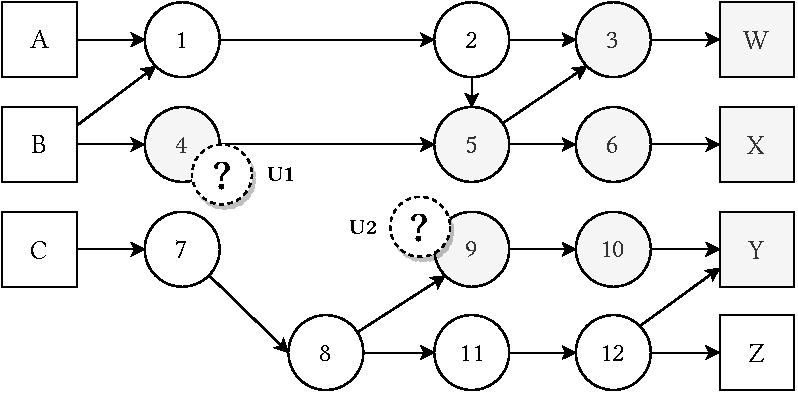
\includegraphics[width=0.8\linewidth]{figures/chapter6/dfd-simple-propagation.pdf}
    \caption{A simple yet versatile \acf*{DFD} with sources (A--C), processes (1--12), sinks (W--Z), and data flows. Uncertainty is denoted by question marks (U1, U2) and the impact set is colored gray.}
    \label{fig:impactanalysis:dfdpropagation:simple}
\end{figure}

\autoref{fig:impactanalysis:dfdpropagation:simple} shows a simplified \ac{DFD} with multiple processes, sources, sinks, and flows, demonstrating the versatility of this notation.
We use this graph instead of the running example because it contains more special cases, e.g., forking and joining data multiple times.
The figure also shows two starting points of the uncertainty propagation, depicted with question marks, named \textbf{U1} and \textbf{U2}.
The annotated nodes represent the starting nodes, i.e., $\var{start_{U1 \cup U2}} = \setted{\var{4,9}}$.
The nodes contained in the impact set are colored gray.
The informally described rule of uncertainty propagation in \acp{DFD} becomes visible here.
Every node that can be reached from the starting nodes is contained in the uncertainty impact set.
In this simplified example, $\var{impact_{U1}} = \setted{3,4,5,6,W,X}$ and $\var{impact_{U2}} = \setted{9,10,Y}$.
Trivially, nodes can also be contained in multiple impact sets if the impact of multiple starting nodes overlaps.
Because the \ac{UIP} does also not affect uncertainty impact analysis in \acp{DFD}, we can merge the impact sets to form the full impact set $\var{impact_{U1 \cup U2}} = \setted{3,4,5,6,9,10,W,X,Y}$.

If we interpret uncertainty as unanticipated change, it can only affect confidentiality at every point that is affected by the change.
Regarding data flows, this requires data to be processed or forwarded by an affected node.
Nodes that have no contact with certain flowing data cannot affect the data's confidentiality, regardless of uncertainty. 
After a data flow has been impacted by uncertainty, we do not make any further assumptions about confidentiality, as any node could or could not violate confidentiality.
In our running example, an uncertain data processing could affect confidentiality directly in the affected processing action, or in a subsequent validation check, or when the data flows to the \emph{Database Service} component, or when the data is stored in the database.
This depends on the modeled software architecture and the specified confidentiality requirements.
However, we can safely exclude any node that cannot be reached by an impacted node following the flow of data.
This includes all previous nodes to the impacted node in the data flow but also all other nodes that cannot be reached.
As software systems usually contain many, independent data flows \cite{seifermann_architectural_2022}, this highly reduces the potential size of the impact set.

\finding{Uncertainty in \acfp{DFD} propagates along data flows, starting from an impacted node until a sink is reached. Preceding nodes and nodes that cannot be reached following the flow of data are not affected.}


\subsection{Formal Foundation for Uncertainty Impact Analysis}

As introduced in \autoref{sec:foundations:dfd} and discussed previously in \autoref{sec:classification:dfd}, \acp{DFD} can be represented using \acp{DAG} \cite{canfora_data_1992}.
Regarding uncertainty impact analysis, we do not require the distinction between primary and secondary uncertainty.
For impact analysis, we only consider \ac{DFD} nodes---or \ac{DAG} vertices---that are either contained or not contained in an impact set.
Thus, we do not alter the \ac{DAG} but only reference a subset of its nodes as an impact set.
We explained these sets at the beginning of this section with \autoref{fig:impactanalysis:dfdpropagation:simple}.

A \ac{DAG} $G = (V, E)$ consist of vertices $V$ and edges $E$.
These represent nodes and data flows, respectively.
Two vertices $u, v \in V$ are strictly partially ordered $v \prec u$ if there exists a path from $v$ to $u$, i.e., a data flow.
This data flow can also be transitive because a strict partial order is irreflexive, asymmetric, and transitive \cite{knuth_art_1997}.
For instance, in \autoref{fig:impactanalysis:dfdpropagation:simple}, $4 \prec 5$ and also $4 \prec 6$ but $4 \nprec B$ and $4 \nprec 9$ because there is no (transitive) data flow.
An induced subgraph $G[V']$ consists of a subset of vertices $V' \subseteq V$ and all edges that have both endpoints in $V'$ \cite{diestel_graph_2017}.
Put simply, in our \acp{DAG}, we start with a vertex and add all vertices that can be reached from this vertex and all the required edges to reach these vertices to the subgraph.
For instance, in \autoref{fig:impactanalysis:dfdpropagation:simple}, $V' = \setted{12, Y, Z}$ induces the subgraph $G' =: G[V']$ with vertices $V'$ and edges $\setted{\flow{12}{Y}, \flow{12}{Z}} = E' \subset E$.

To propagate uncertainty in \acp{DFD}, we start with a vertex $v \in V$ and add it to the impact set $S \subseteq V$.
Then, we iteratively add all vertices that are in the direction of the data flow, i.e., all $u \in V$ where $v \prec u$.
We add all visited edges to the subset $E' \subseteq E$.
The propagation ends once we reached all reachable data sinks, i.e., vertices without outgoing edges.
$S$ then induces a subgraph $G[S]$ with all impacted vertices and all directed edges $E'$ between them.
This subgraph itself forms a \ac{DAG} $G' = (S,E')$.
Note that we do not limit the size of $S$.
In severe cases and wide uncertainty impacts, $S = V$.

In our current example introduced in \autoref{fig:impactanalysis:dfdpropagation:simple}, these induced subgraphs are represented by the nodes that are colored gray.
Uncertainty \textbf{U1} causes the induced subgraph $G_{U1} =: G[S_{U1}]$ with $S_{U1} = \setted{3, 4, 5, 6, W, X}$ and edges $E_{U1} = \setted{\flow{4}{5}, \flow{5}{3}, \flow{5}{6}, \flow{3}{W}, \flow{6}{X}}.$
Uncertainty \textbf{U2} causes the induced subgraph $G_{U2} =: G[S_{U2}]$ with $S_{U2} = \setted{9, 10, Y}$ and edges $E_{U2} = \setted{\flow{9}{10},\flow{10}{Y}}$.
$S_{U1}$ and $S_{U2}$ represent the impact sets presented in the beginning of this section.
They also represent the final impact set of uncertainty regarding confidentiality, i.e, the result of our uncertainty impact analysis.
Note that impact sets can be a subset of another impact set as well as the induced subgraphs can be subgraphs of other induced subgraphs.
Due to our construction of induced subgraphs, both conditions imply each other.
For instance, for the a subgraph $G[V'']$ induced by $V'' = \setted{10,Y}$ with the edge $\setted{\flow{10}{Y}}$, we see $V'' \subset S_{U2}$ and $G[V''] \subseteq G_{U2}$.

\finding{The impact of uncertainty in \acfp{DAG} follows the strict partial order of the data flow.
Uncertainty impact sets contain the affected vertex and all vertices that can be reached via directed edges.
They induce subgraphs of the \ac{DAG} representing the uncertainty impact.}


\subsection{Algorithm for Uncertainty Impact Analysis in Data Flow Diagrams}

Based on the findings presented above, we define an algorithm for uncertainty impact analysis in \acp{DFD}.
Here, we see the benefits of using simple graphs like \acp{DAG} for the propagation.
Due to the lack of cycles, we can apply simplified versions of \acf{DFS} or \acf{BFS} \cite{knuth_art_1997} without the need for testing for already visited vertices.
The resulting sets represent the final impact sets without further steps required regarding the propagation. 
They can be used to induce subgraphs of the \ac{DAG}.

\begin{algorithm}
    \caption{Algorithm for uncertainty propagation in data flow diagrams}
    \label{alg:impactanalysis:dfd}
    \begin{algorithmic}[1] 
        \Procedure{\function{propagateUncertaintyInDFD}}{$\var{start}, \var{graph}$}
            \algindentskip
            \State $\var{stack} \gets \sequenced{\var{start}}$ \Comment{Initialize stack with the start vertex} \label{alg:impactanalysis:dfd:2}
            \State $\var{impactset} \gets \emptyset$ 
            \algblockskip

            \While{$\function{notEmpty}(\var{stack})$} \label{alg:impactanalysis:dfd:4}
                \State $\var{vertex} \gets \function{pop}(\var{stack})$
                \State $\var{impacset} \gets \var{impactset} \cup \setted{\var{vertex}}$ \Comment{Fill the impact set} \label{alg:impactanalysis:dfd:6} 
                \For{$successor \in \function{getSuccessors}(\var{vertex}, \var{graph})$} \label{alg:impactanalysis:dfd:7}
                    \State $\function{push}(\var{stack}, \var{successor})$
                \EndFor
            \EndWhile
            \algblockskip

            \State \Return{$\var{impactset}$} \label{alg:impactanalysis:dfd:11}
            \algindentskip
        \EndProcedure
    \end{algorithmic}
\end{algorithm}

\autoref{alg:impactanalysis:dfd} shows the algorithm for uncertainty propagation in \acp{DFD}.
We first initialize the stack used for the search and the resulting impact set, starting in \autoref{alg:impactanalysis:dfd:2}.
While the stack is not empty, we add the identified vertices to the impact set in \autoref{alg:impactanalysis:dfd:6} and continue with all neighbors in the direction of the data flow, i.e., all successors in \autoref{alg:impactanalysis:dfd:7}.
The stack runs empty when no further vertices can be found, i.e., when we have found all reachable data sinks.
Last, the resulting impact set is returned in \autoref{alg:impactanalysis:dfd:11}.

We discussed the one-to-many relation between an uncertainty source and its impact in \autoref{sec:impactanalysis:representing}.
While this relation becomes visible already in the architectural propagation, it is common in the data flow-based propagation.
If at least one vertex is affected by uncertainty that is not a data sink, the number of impacted elements grows larger than the number of annotated elements.
Based on this graph-oriented point of view, we can see again the need for uncertainty impact analysis to understand the potential impact of uncertainty on confidentiality.





\section{Uncertainty Impact Analysis regarding Confidentiality}%
\label{sec:impactanalysis:impactanalysis}

We combine the propagation of uncertainty in architectural models with the propagation of uncertainty in \acp{DFD} to complete our uncertainty impact analysis regarding confidentiality.
On the one hand, the architectural propagation uses modeled information to retrieve the uncertainty impact that is missing in \acp{DFD}.
On the other hand, the architectural propagation, which is based on change impact analysis \cite{rostami_architecture-based_2015,rostami_architecture-based_2015,busch_architecture-based_2020}, requires handling special cases, has more complex propagation rules, and is specific to concrete \acp{ADL} like the \ac{PCM}.
Uncertainty propagation in \acp{DFD} is \ac{ADL}-independent and can easily be defined based on \ac{DFS} or \ac{BFS}.
Thus, we connect both impact analyses to combine their benefits.
This concludes our approach to address Problem \PR{2}{2}.

To achieve this, we reuse the mapping of \ac{PCM} to \acp{DFD}, defined by \textcite{seifermann_architectural_2022}.
We first calculate the partial impact set of the architectural uncertainty impact analysis.
This impact set consists of different elements of the \ac{PCM}, namely \emph{StartActions}, \emph{StopActions}, \emph{SetVariableAction}, and \emph{ExternalCallActions} that are described in \acp{SEFF} and also \emph{EntryLevelSystemCalls} that are specified in the \emph{UsageScenario}.
All of these actions have counterparts in the extracted \acp{DFD} and there is a one-to-one mapping between these actions and their corresponding \ac{DFD} nodes.
This satisfies the relation presented in \autoref{fig:impactanalysis:representing:relation} as every \ac{DFD} node is a unique origin in the architectural model.


\subsection{Coupling the Uncertainty Impact Analysis Approaches}

We extend the notation introduced in \autoref{sec:impactanalysis:dfdpropagation} to present the coupled analyses.
We use \acp{DAG} $G = (V, E)$ to represent \acp{DFD} with the strict partial order $u, v \in V, u \prec v$ representing data flows.
Let $A = \setted{a_{1},\dots,a_{n}}$ be the set of all architectural elements like components, or interfaces and let $S = \setted{s_{1},\dots,s_{n}}$ be the set of all uncertainty sources.
We name the annotation of an uncertainty source to an architectural element $a : S \rightarrow A$.
For instance, in our running example, $\setted{\var{PurchaseInterface}, \var{processUserData}} \subset A$, and $S = \setted{\var{U1}, \var{U2}, \var{U3}, \var{U4}}$.
Then, we can specify the annotations as $a(\var{U1}) = PurchaseInterface$, or $a(\var{U4}) = CloudService$, as shown in \autoref{table:impactanalysis:sisexample}.
We reuse the mapping \cite{seifermann_architectural_2022} from an architectural element to its corresponding vertices of the \ac{DFD} as $m : A \rightarrow V$.

The uncertainty impact analysis can be defined as function $u : S \rightarrow X \subseteq V$, where $S$ represents all uncertainty sources.
$X$ induces a subgraph $G[X]$ of the \ac{DFD}, i.e., the part of the software system that is affected by the annotated uncertainty sources. 
The analysis consists of three steps:
First, we conduct the architectural propagation of the uncertainty based on the  by adapting the propagation rules defined by change impact analysis.
For example, altering an interface does affect both its caller and the callee.
We define the architectural propagation as $p_{A} : A \rightarrow A$.
Second, we apply the previously defined mapping $m : A \rightarrow V$ from all affected architectural elements to their corresponding vertices of the \ac{DFD}.
Third, we define the propagation along the data flow as $p_{D} : V \rightarrow X \subseteq V$.
The previously mapped vertices represent the first affected nodes in the direction of the data flow, so that $\forall x \in X \subseteq V, \exists a \in A : m(a) = x \vee m(a) \prec x$.
The induced subgraph $G[X]$ represents the full impact set including transitive effects.
In sum, we define the uncertainty impact analysis as $u = p_{D} \circ m \circ p_{A} \circ a$.

Put simply, starting with the annotation function $a$, we receive all annotated elements of the software architecture, e.g., the \emph{PurchaseInterface}.
The architectural propagation $p_{a}$ yields all impacted elements of the software architecture, e.g., the \emph{EntryLevelSystemCall} to purchase items.
We apply the mapping $m$ to find the \ac{DFD} node corresponding to this \emph{EntryLevelSystemCall}.
Then, we use the data flow-based propagation $p_{D}$ to identify all nodes where data from this node flows.
Speaking in terms of \acp{DAG}, these represent a subset of all vertices $X \subseteq V$ that induce a subgraph of the \ac{DAG}.
This represents the final result of the uncertainty impact analysis, showing the potential impact of uncertainty on the software system regarding confidentiality.


\subsection{Algorithm for the Coupled Uncertainty Impact Analysis}

\begin{algorithm}
    \caption{Algorithm for uncertainty impact analysis regarding confidentiality}
    \label{alg:impactanalysis:impactanalysis}
    \begin{algorithmic}[1] 
        \Procedure{\function{propagateUncertainty}}{$\var{uncertainty}, \var{model}$}
            \algindentskip
            \State $\var{candidates} \gets \emptyset$ \label{alg:impactanalysis:impactanalysis:2}
            \algblockskip

            \Switch{$\function{typeOf}(\var{uncertainty})$} \Comment{Propagation in the architectural model $p_{A}$} \label{alg:impactanalysis:impactanalysis:3}
                \Case{$\datatype{ComponentUncertainty}$}
                    \State $candidates \gets \function{propagateComponentUncertainty}(\var{uncertainty}, \var{model})$
                \EndCase
                \Case{$\datatype{InterfaceUncertainty}$}
                    \State $candidates \gets \function{propagateInterfaceUncertainty}(\var{uncertainty}, \var{model})$
                \EndCase
                \Case{$\datatype{ConnectorUncertainty}$}
                    \State $candidates \gets \function{propagateConnectorUncertainty}(\var{uncertainty}, \var{model})$
                \EndCase
                \Case{$\datatype{ExternalUncertainty}$}
                    \State $candidates \gets \function{propagateExternalUncertainty}(\var{uncertainty}, \var{model})$
                \EndCase
                \Case{$\datatype{BehaviorUncertainty}$}
                    \State $candidates \gets \function{propagateBehaviorUncertainty}(\var{uncertainty}, \var{model})$
                \EndCase
            \EndSwitch
            \algblockskip

            \State $\var{impactset} \gets \emptyset$ \Comment{Mapping to the data flow diagram $m$}
            \State $\var{graph} \gets \function{mapToDataFlowDiagram}(\var{model})$ \label{alg:impactanalysis:impactanalysis:15}
            \State $\var{candidates} \gets \function{mapToVertices}(\var{candidates}, \var{model}, \var{graph})$ \label{alg:impactanalysis:impactanalysis:16}
            \algblockskip

            \For{$\var{vertex} \in \var{candidates}$} \Comment{Propagation in the data flow diagram $p_{D}$} \label{alg:impactanalysis:impactanalysis:17}
                \State $\var{impactset} \gets \var{impactset} \cup \function{propagateUncertaintyInDFD}(\var{vertex}, \var{graph})$
            \EndFor
            \algblockskip

            \State \Return{$\var{impactset}$} \label{alg:impactanalysis:impactanalysis:20}
            \algindentskip
        \EndProcedure
    \end{algorithmic}
\end{algorithm}

This foundation enables the combination of uncertainty impact analysis in architectural models and \acp{DFD}.
\autoref{alg:impactanalysis:impactanalysis} shows the resulting propagation algorithm for analyzing the impact of uncertainty on confidentiality in \ac{PCM} models.
This algorithm combines all algorithms that have been introduced in \autoref{sec:impactanalysis:pcmpropagation} and \autoref{sec:impactanalysis:dfdpropagation} and realizes the aforementioned coupling of the uncertainty impact analysis approaches.

We start with an empty set of candidates in \autoref{alg:impactanalysis:impactanalysis:2}.
Depending on the type of the annotated uncertainty source, we choose the matching algorithm for the architectural propagation in \autoref{alg:impactanalysis:impactanalysis:3}.
This represents the function $p_{A}$.
The result of this propagation is one or more elements from the architectural model, i.e., \ac{PCM} elements.
Which and how many candidate elements are identified in the architectural propagation depends on the architectural model and the type of uncertainty.
For instance, \emph{Behavior} uncertainty yields one element in most of the cases, as specified in \autoref{alg:impactanalysis:behavior}.
On the contrary, \emph{Interface} uncertainty always yields multiple candidate elements, as described in \autoref{alg:impactanalysis:interface}.

Afterward, we map the architectural model to a \ac{DFD} and all candidate elements to their corresponding vertices, starting in \autoref{alg:impactanalysis:impactanalysis:15}.
We do not elaborate the functions \emph{mapToDataFlowDiagram} and \emph{mapToVertices} but refer to the definition of this mapping \cite{seifermann_data-driven_2019,seifermann_architectural_2022} and to the examples provided in \autoref{fig:runningexample:dfd} and \autoref{fig:impactanalysis:representing:example}.
The result of this mapping in \autoref{alg:impactanalysis:impactanalysis:16} is a set of vertices representing the starting points for the uncertainty impact analysis in \acp{DFD}.
This represents the function $m$.
We propagate the uncertainties in the \acp{DFD}, starting in \autoref{alg:impactanalysis:impactanalysis:17}.
We have to repeat this step for every candidate vertex as there can be multiple candidates.
The impact set is the union of all individual propagation results.
This represents the function $p_{D}$.
The final impact set is returned in \autoref{alg:impactanalysis:impactanalysis:20}.


\subsection{Applying Uncertainty Impact Analysis Regarding Confidentiality}

\begin{table}
    \centering
    \begin{tabular}{lp{1.8cm}ll}
        \toprule
         & Annotated element & \mtl{Affected \ac{PCM} elements,\\Mapped \ac{DFD} nodes} & Uncertainty Impact set\\
        \midrule
        \mtl{\U{1}} & \mtl{Purchase-\\Interface} & \mtl{PurchaseInterface.purchaseItem,\\purchaseItem.start}
            & \mtl{PurchaseInterface.purchaseItem,\\purchaseItem.start,\\processPurchase,\\processUserData,\\\dots}\\
        \midrule
            \U{2} & \mtl{process-\\UserData} & \mtl{processUserData }
            & \mtl{processUserData,\\DBService.storePurchaseData,\\storePurchaseData.start,\\storeData,\\\dots}\\
        \midrule
            \U{3} & \mtl{Database-\\Service} & \mtl{queryInventory.start,\\storePurchaseData.start} 
            & \mtl{queryInventory.start,\\queryData,\\Database,\\returnData,\\\dots}\\
        \midrule
            \U{4} & \mtl{Cloud-\\Service} & \mtl{queryInventory.start,\\queryData,\\storeData,\\\dots} 
            & \mtl{queryInventory.start,\\queryData,\\Database,\\returnData,\\\dots}\\
        \bottomrule
    \end{tabular}
    \caption{Shortened results of all steps of the uncertainty impact analysis regarding confidentiality.}%
    \label{table:impactanalysis:runningexample}
\end{table}

To exemplify the full uncertainty impact analysis, we apply it to the running example introduced in \autoref{ch:runningexample}.
This example contains four uncertainty sources that demonstrate different uncertainty types, namely \emph{Connector} uncertainty (\U{1}), \emph{Behavior} uncertainty (\U{2}), \emph{Component} uncertainty (\U{3}), and \emph{External} uncertainty (\U{4}).
In the first step, software architects annotate the model with these uncertainty sources, as described in \autoref{fig:overview:procedure}.
This represents the annotation function $a$.
We showed exemplary annotation targets, i.e., elements from the \ac{PCM} model in \autoref{table:impactanalysis:sisexample} and repeat them in \autoref{table:impactanalysis:runningexample} for convenience.

Afterward, \autoref{alg:impactanalysis:impactanalysis} propagates the annotated uncertainty sources within the architectural model, using the propagation algorithm that fits the annotated uncertainty.
This represents the architectural uncertainty impact analysis $p_{A}$.
We showed exemplary propagation results, i.e., elements of the software architecture that could be affected by the annotated uncertainty in \autoref{sec:impactanalysis:pcmpropagation} and summarize them in \autoref{table:impactanalysis:runningexample}.

The affected elements of the software architecture are mapped to corresponding \ac{DFD} nodes.
To achieve this, we use the tracing information from the extraction of \acp{DFD} based on the mapping of \textcite{seifermann_architectural_2022}.
Every \ac{DFD} node has an origin within the \ac{PCM} model, see \autoref{fig:impactanalysis:representing:relation}.
This represents the mapping function $m$.
We show the results of this mapping in \autoref{table:impactanalysis:runningexample}.
Note that the nodes' names are identical to elements of the software architecture.
This is not by accident but to simplify the later identification of uncertainty-afflicted elements and confidentiality violations.

Last, we propagate the uncertainty within in the \ac{DFD}, starting at each vertex retrieved from the mapping of affected architecture elements, as shown in \autoref{alg:impactanalysis:impactanalysis}.
This represents the uncertainty impact analysis in \acp{DFD} $p_{D}$.
The result of this analysis step is the final uncertainty impact set that is shown to the software architect.
We shorten the results of this step in \autoref{table:impactanalysis:runningexample}.
The full impact set can be found in \autoref{sec:appendix:impactset}.

\begin{figure}
    \centering
    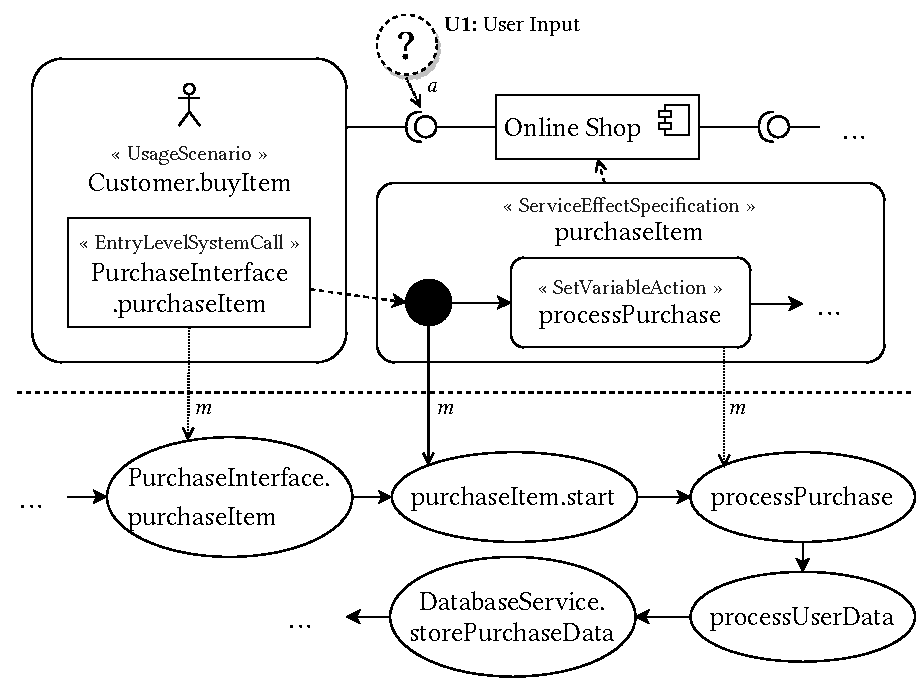
\includegraphics[width=0.9\linewidth]{figures/chapter6/impact-runningexample.pdf}
    \caption{Informal illustration of the propagation of an uncertainty source in the architectural model (top) and a \acf*{DFD} (bottom) using the annotation function a and the mapping function m.}
    \label{fig:impactanalysis:runningexample}
\end{figure}

To illustrate the propagation path of an uncertainty source, \autoref{fig:impactanalysis:runningexample} informally shows the propagation of Uncertainty \U{1}.
We chose this uncertainty source as it is annotated to the \emph{Customer} of the \emph{Online Shop} and thus has the longest path until it reaches a data sink.
For the sake of brevity, we leave out many details and focus only on the propagation path.
The full example can be found in our data set \cite{dataset}, and in \autoref{sec:appendix:impactset}.
Uncertainty \U{1} represents the user input and is annotated to a \emph{ProvidedDelegationConnector} called \emph{PurchaseInterface}.
It propagates to an \emph{EntryLevelSystemCall} in the \emph{UsageScenario} named \emph{Customer.buyItem} and to the \emph{StartAction} of a \ac{SEFF} in the architectural model.
The actions are mapped to \ac{DFD} nodes.
Afterward, the uncertainty is propagated in the \ac{DFD} until a sink is reached.
All \ac{DFD} nodes are part of the impact set of Uncertainty \U{1}.  


\subsection{Tool Support for Uncertainty Impact Analysis}

In the introduction of this chapter, we discussed the need for automated analyses to aid the software architectural design process.
Manual propagation of uncertainty is not feasible, especially in large systems of systems with hundreds of architectural elements or \ac{DFD} nodes \cite{hahner_architecture-based_2023}.
This need for automated analysis is also described in Problem \PR{2}{2}.

We realize the algorithms described in this chapter as part of our tooling \uia.
Here, we build on the Palladio tooling \cite{reussner_modeling_2016,reussner_palladio_2024} that offers a meta model, the \ac{PCM}, and graphical editor support.
Our Java-based open-source implementation of the propagation logic is integrated into the Eclipse-based tooling, and part of the data set \cite{dataset}.

\begin{figure}
\begin{lstlisting}[
    style=demo,
    caption={Shortened output of the uncertainty impact analysis showing the impact of Uncertainty U2.},
    label={lst:impactanalysis:result}
]
    Behavior Uncertainty Impact on SEFFActionSequenceElement with 
        ID _oEBNYDIXEe-m4c0ChzWfPg (represeting a SetVariableAction).
    Origin of this impact: Behavior Uncertainty annotated to 
        SetVariableAction "UserDataProcessing" (_oEBNYDIXEe-m4c0ChzWfPg).

    All affected elements (1):
    SEFFActionSequenceElement (UserDataProcessing, _oEBNYDIXEe-m4c0ChzWfPg)

    Impact set (1):
    0: SEFFActionSequenceElement (UserDataProcessing)
    CallingSEFFActionSequenceElement / calling (DatabaseStoreInventory)
    SEFFActionSequenceElement (Beginning updateInventory)
    SEFFActionSequenceElement (Ending updateInventory)
    CallingSEFFActionSequenceElement / returning (DatabaseStoreInventory)
    ...
\end{lstlisting}
\end{figure}

Here, we included many of the already discussed optimization strategies to speed up the propagation, e.g., by caching query results or using the extracted \ac{DFD} to filter affected architecture elements.
Using this approach, all propagation algorithms can be realized as \ac{DFS}, which is in $\mathcal{O}(V + E)$, where $V$ represents the \ac{DFD} nodes and $E$ represents the edges \cite{knuth_art_1997}.
Put simply, we test for each node whether or not it is affected by uncertainty, and then propagate the uncertainty along the data flow.

Software architects annotate uncertainty sources by calling the analysis interface and providing the element's identifier.
The analysis performs a type check to ensure the validity of the annotation and then propagates the uncertainty without requiring any further user interaction.
The result comprises the annotated elements, the affected elements in the \ac{PCM} model, and the complete impact set.
\autoref{lst:impactanalysis:result} shows an exemplary but shortened output of \uia for Uncertainty \U{2} with uncertainty type, annotation target, and analysis results.
The full output can be found in \autoref{sec:appendix:impactset}.
This output can be used to further enhance the display of the impact, e.g., by highlighting affected areas of \acp{DFD} in graphical viewers or editors \cite{boltz_extensible_2024}.

We also implemented additional processing to enhance the user experience.
As discussed in \autoref{sec:impactanalysis:dfdpropagation}, impact sets of uncertainty sources can be a subset of impact sets of other uncertainty sources.
In our running example, the impact set of \U{2} is a subset of the impact set of \U{1} because it affects a subgraph of the \ac{DAG} representing the user input's processing.
We identify such relations and only return the largest impact sets that are not subsets of another subset.
Formally speaking, the analysis yields an antichain \cite{diestel_graph_2017} with the partial order of the subset relation, in which all impact sets are pairwise incomparable.

\finding{The uncertainty impact analysis can be fully automated based on the \acf{PCM} and the existing tooling of the Palladio approach.
Propagating uncertainty requires minimal additional effort by software architects, as the analysis only requires annotating uncertainty sources.
}





\section{Addressing the Uncertainty Awareness Problem}%
\label{sec:impactanalysis:awareness}

Our approach to uncertainty impact analysis supports software architects in the early assessment of the impact of uncertainty on confidentiality.
However, it suffers from the \acf{UAP}, like many other uncertainty-aware analyses \cite{hezavehi_uncertainty_2021}.
As introduced in \autoref{sec:classification:identification}, the \ac{UAP} hinders the analysis of uncertainty due to the lack of knowledge about relevant uncertainty sources.
Failing the correct identification, classification, and annotation limits the validity of analysis results, as they can lack both precision and comprehensiveness.
In this section, we demonstrate how to tackle this problem regarding our uncertainty impact analysis.
We connect \arcen, which was introduced in \autoref{sec:classification:collaboration}, to our impact analysis tooling \uia.
This addresses Problem \PR{2}{3} and is a step toward end-to-end analysis approaches \cite{weyns_towards_2023}.

To tackle the \ac{UAP} in uncertainty impact analysis, we need to solve two underlying problems.
First, the analysis and its tooling must receive information about relevant uncertainty sources and their classification.
Second, software architects operating the analysis must become aware of potential sources and identify appropriate annotation targets.
Both problems arise before the automated analysis is performed.
Thus, we extend the uncertainty impact analysis by an additional identification step prior to the propagation.

After our tooling \uia has been initialized and all \ac{PCM} models are loaded, we request a current list of uncertainty sources from \arcen.
This is possible because \arcen provides the uncertainty source catalog in a machine-readable format, as presented in \autoref{sec:classification:collaboration}.
This catalog also includes the classification of each source, as shown with the underlying meta model in \autoref{fig:classification:identification:metamodel}.
Software architects use \arcen to identify relevant uncertainty sources.
As all uncertainty sources in the uncertainty source catalog have a unique identifier, they can provide this identifier to the extended impact analysis.
After resolving the uncertainty source and the classification category \emph{Architectural Element Type}, the analysis queries all \ac{PCM} models to identify matching annotations targets.
These are displayed to the software architects in an interactive interface.

\begin{figure}
\begin{lstlisting}[
    style=demo,
    caption={Exemplary interaction of a software architect with the extended uncertainty impact analysis.},
    label={lst:impactanalysis:awareness}
]
    Enter an id of an uncertainty to check for:
    > #48

    Select one of these elements.
    1) "OnPremiseServer" (_qvz80ITgEeywmO_IpTxeAg)
    2) "CloudServer" (_upfkIITgEeywmO_IpTxeAg)

    Enter line number:
    > 2

    Analysis completed. Result:
    ...
\end{lstlisting}
\end{figure}

\autoref{sec:impactanalysis:awareness} shows an exemplary interaction prior to the propagation of uncertainty.
In the running example, we have two \emph{ResourceContainers} that can be affected by uncertainty about the provider's trustworthiness (\U{4}), represented as uncertainty number 48 in \arcen.
After annotating this uncertainty source to the \emph{CloudServer}, the uncertainty impact analysis is executed.
The full result, including the impact set, is returned, similar to \autoref{lst:impactanalysis:result}.

This addresses the \ac{UAP} by providing software architects with a list of possible uncertainty sources to choose from.
Additionally, less expert knowledge about the classification is required as the interpretation is done automatically.
Last, the manual effort of searching the architectural model to identify potential elements to annotate with uncertainty is reduced.
In sum, this demonstrates the feasibility of extending an existing analysis, even without altering the core propagation algorithms.
We stress that other uncertainty-aware analyses \cite{hahner_model-based_2023,walter_architectural_2022,walter_architecture-based_2023} could similarly benefit from such extension.

\finding{By connecting the identification and classification of uncertainty to model-based uncertainty analysis, the \acf{UAP} can be addressed.
Although this does not fully resolve the challenge of unanticipated change, it reduces the severity.
Approaches like this represent a step toward the end-to-end analysis of uncertainty.}





\section{Uncertainty Propagation in Uncertainty Flow Diagrams}%
\label{sec:impactanalysis:ufd}

We conclude this chapter by discussing the generalization of the presented concepts to tackle related problems from the community of \acp{SAS} \cite{weyns_towards_2023}.
In the recent past, the \acf{UIP} has received increased attention \cite{camara_addressing_2022,camara_uncertainty_2022,weyns_towards_2023}.
This problem arises because uncertainties in software-intensive systems are rarely independent \cite{camara_uncertainty_2022}.
Addressing this problem goes beyond handling single uncertainty sources but poses additional challenges regarding modeling, analysis, and mitigation \cite{camara_addressing_2022}.
Handling the \ac{UIP} requires notations to represent and analyze the interaction of \emph{heterogeneous} uncertainty sources, i.e., uncertainty that differs in type and nature.
Additionally, this notation must support horizontal propagation in the same level of abstraction, and vertical propagation across abstraction levels.
This is also summarized in Problem \PR{2}{4}.

Uncertainty propagation has been identified early as a possible approach towards handling uncertainty interactions \cite{camara_addressing_2022}.
However, the few existing approaches tackling uncertainty propagation focus on \emph{homogeneous} uncertainties, i.e., uncertainties that are similar in nature, admit the same representations and are amenable to similar reasoning mechanisms \cite{camara_uncertainty_2024}.
In the following, we build on the knowledge about uncertainty propagation in \acp{DFD}, previously presented in this chapter.
We define a new notation called \acf{UFD} that enables the representation and propagation of heterogeneous uncertainty sources.
Thereby, we generalize the propagation concept introduced in this chapter and make a first step towards comprehensive modeling and analysis of the \ac{UIP}\footnote{When I presented the research about uncertainty propagation regarding confidentiality at SEAMS '23, I was asked by Danny Weyns about the application of these concepts to \acp{SAS}. My answer comprised the application of models at runtime and the integration into the analysis phase of \acs{MAPEK}. However, in hindsight, \acfp{UFD} would have been the perfect answer.}.

In our running example, we see an uncertainty interaction between Uncertainty \U{3} and \U{4}.
We discussed this interaction when we introduced the difference between primary and secondary uncertainty in \acp{DAG} in \autoref{sec:classification:dfd}.
If Uncertainty \U{3} resolves to a deployment location that is not in the cloud, Uncertainty \U{4} about the cloud provider has no effect.
Otherwise, the combination of both uncertainty sources is relevant.
This represents a simple uncertainty interaction where the outcome can be understood by investigating all possible scenarios.
However, other interactions could lead to results that go further and introduce new and unanticipated changes \cite{camara_addressing_2022,camara_uncertainty_2024}.
An example is Znn.com \cite{cheng_evaluating_2009}, where uncertainty about the sensor input interacts with the discretization of the input.
Here, the interaction of both uncertainties can lead to false adaption, although both uncertainty sources on their own would not have affected the system behavior \cite{camara_uncertainty_2024}.

\begin{figure}
    \centering
    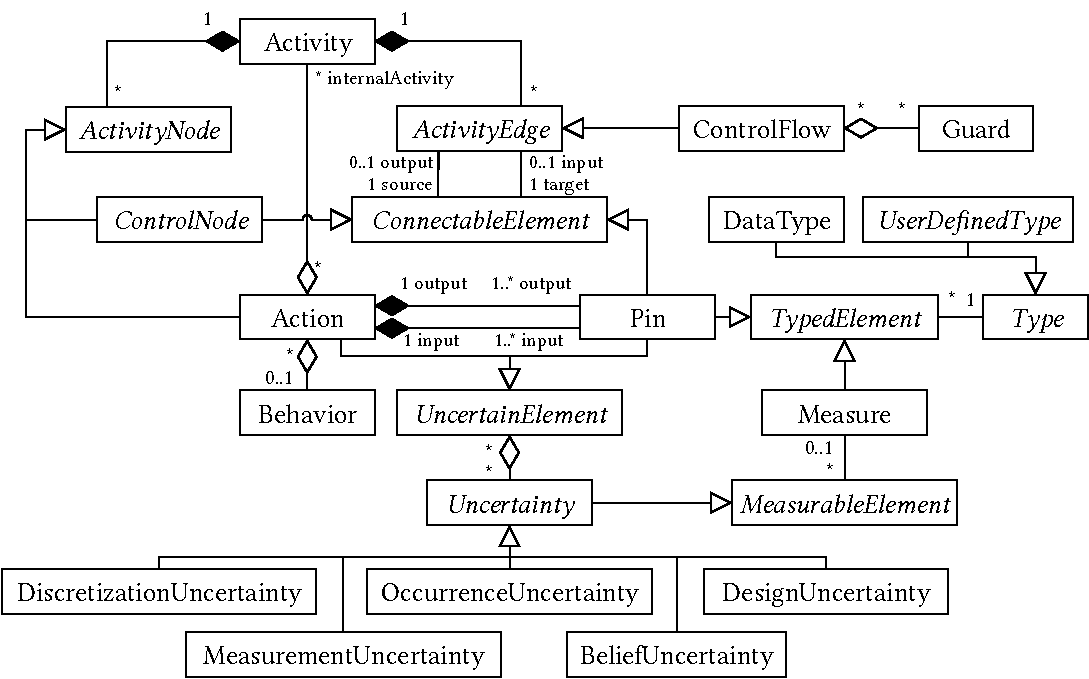
\includegraphics[width=\linewidth]{figures/chapter6/ufd.pdf}
    \caption{Simplified meta model of the \acf*{UFD} notation.}
    \label{fig:impactanalysis:ufd}
\end{figure}

\autoref{fig:impactanalysis:ufd} shows the simplified \ac{UFD} meta model \cite{camara_uncertainty_2024}.
This represents a simplified version of \acp{DFD} \cite{demarco_structure_1979} or \ac{UML} activity diagrams \cite{object_management_group_unified_2015}, extended with information about uncertainty, based on \ac{PSUM} \cite{PSUM}.
The top-level element is the \emph{Activity}, i.e., a graph whose nodes and edges are \emph{ActivityNodes} and \emph{ControlFlows}, respectively. 
The graph represents how the information flows through the computations performed by a program. 
\emph{Actions} represent behavior. 
\emph{Actions} are represented by squares with rounded corners and have \emph{Pins} (small white squares) that represent the types of input/output parameters. Each \emph{Pin} has a \emph{Type}.
\emph{Actions} may have an associated \emph{Behavior}, such as the invocation of a method that implements the behavior to transform the action's inputs into outputs.
This approach is similar to the unified modeling primitives \cite{seifermann_unified_2021}.

To enable hierarchical modeling and vertical uncertainty propagation, each \emph{Action} can also be refined by one or multiple \emph{Activities} that represent its inner workings. 
At the highest abstraction level, the whole system can be represented by a single node with input and output pins, i.e., a black box.
Either a \emph{Behavior} or a set of refining internal \emph{Activities} can be specified for an \emph{Action}, but not both.
It is also possible to specify multiple internal activities that represent alternatives.
This enables the expression of structural uncertainty as variations, which is common to represent design uncertainty \cite{troya_uncertainty_2021}.

A \emph{ControlFlow} is represented by a directed arrow that connects the outgoing \emph{Pin} of an \emph{Activity} with the incoming \emph{Pin} of another \emph{Activity}. 
\emph{ControlFlows} may include \emph{Guards} that have to be satisfied for the information to flow between the connected \emph{Pins}, or \emph{ControlNodes}. 
When more than one \emph{Guard} is specified, they all need to be satisfied for the \emph{ControlFlow} to take place.
\acp{UFD} enable the explicit representation of uncertainty, with the goal of dealing with the interactions between uncertainties that happen when making computations. 
\acp{UFD} allow the specification of individual uncertainties associated with \emph{Pins} or with \emph{Actions}. 
Each uncertainty can be of a different type.
This includes the common uncertainty types \emph{Measurement Uncertainty}, \emph{Discretization Uncertainty}, \emph{Occurrence Uncertainty}, \emph{Design Uncertainty}, and also \emph{Belief Uncertainty} \cite{troya_uncertainty_2021}.
Note that these types differ from the uncertainty types when only focusing on confidentiality.
Each uncertainty can have an associated \emph{Measure}, which also has a \emph{Type}. 
One way to assess a \emph{Measurement Uncertainty} is in terms of the accuracy of the measurement, which is normally expressed by means of a real number that represents the possible variation of the nominal value of the parameter, i.e., its estimated standard deviation. 
\emph{Belief Uncertainty} is normally expressed by a real number between 0 and 1 representing the likelihood that the stated fact is true, expressed as a probability.
Alternatively, uncertainty can be expressed by defining multiple \emph{Internal Activities} as a variation of the behavior of a single \emph{Action} which is used to express \emph{Design Uncertainty}.
This also enables the expression of additional uncertainty types if they can be denoted either quantitatively using an associated \emph{Measure} or structurally using alternative internal \emph{Activities}.

\begin{figure}
    \centering
    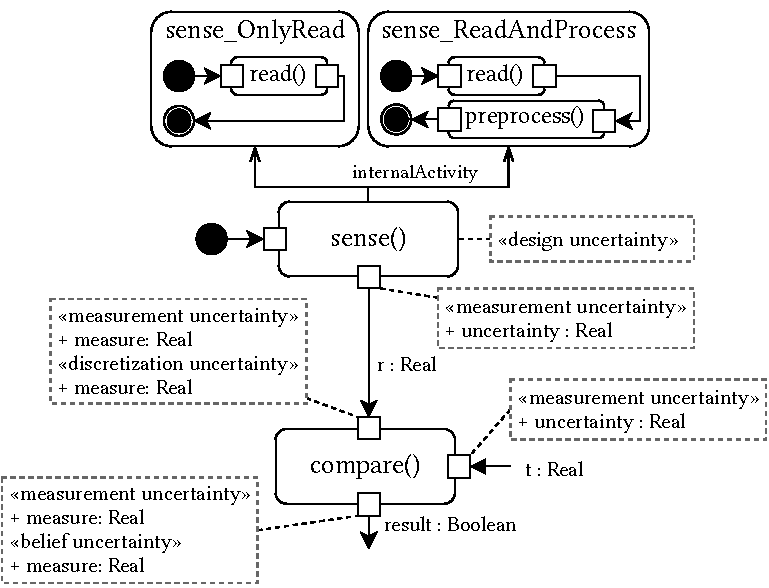
\includegraphics[width=0.8\linewidth]{figures/chapter6/ufd-example.pdf}
    \caption{An \acf*{UFD} showing heterogeneous uncertainty sources and hierarchical modeling.}
    \label{fig:impactanalysis:ufdexample}
\end{figure}

\autoref{fig:impactanalysis:ufdexample} shows an exemplary \ac{UFD}.
The \emph{compare} \emph{Action} compares a sensor value \emph{r} to a threshold \emph{t} to decide whether or not the adaption is triggered.
As described previously, both values are affected by \emph{Measurement Uncertainty}.
The input \emph{r} is additionally affected by \emph{Discretization Uncertainty}, and the uncertain correctness of the \emph{result} is thus subject to \emph{Belief Uncertainty}.
These uncertainties are attached to the matching \emph{Pins} and can be expressed using \emph{Measures}, e.g., the degree of belief, or the variation of the measurement \cite{PSUM}.
Additionally, this example shows \emph{Design Uncertainty} in the \emph{sense} \emph{Action}.
Here, two versions are possible, depending on whether additional preprocessing is used.
This can affect the \emph{Measurement Uncertainty} in \emph{r} and is represented using \emph{Internal Activities}.

In sum, this notation enables the expression of heterogeneous uncertainty sources and their propagation, both horizontally and vertically.
Thereby, \acp{UFD} are still close to the unified modeling primitives \cite{seifermann_unified_2021} or \acp{DFD}\footnote{This research started at the 2023 Bertinoro research seminar on uncertainty in \acp{SAS}. Our group consisted of Javier Camara, Diego Perez-Palacin, Antonio Vallecillo, Maribel Acosta, Nelly Bencomo, Radu Calinescu, Simos Gerasimou, and myself. After discussing the \acf{UIP} for days, we were surprised how concise \acfp{UFD} can be.}.
The propagation of uncertainty in \acp{UFD} is similar to the propagation in \acp{DFD}, i.e., following all edges of a node until a sink is reached.
Although \acp{UFD} are a promising approach to generalize the propagation concept to analyze more than confidentiality, this still represents an early proposal \cite{weyns_towards_2023}.
Future research in this direction is required to create comprehensive and tool-supported modeling and analysis approaches to address the \ac{UIP}.





\section{Assumptions and Limitations}%
\label{sec:impactanalysis:limitations}

In this section, we discuss the assumptions and limitations of the different approaches to uncertainty propagation and impact analysis presented in this chapter.
We also provide our reasoning on whether limitations can become critical when applying the approaches.

\paragraph{Using data flow diagrams}
We use \acp{DFD} to investigate confidentiality as proposed by other work \cite{seifermann_detecting_2022,sion_security_2020,schneider_how_2024}.
Although this simplifies the propagation algorithms and provides a widely used and well-known foundation for our work, it limits the generalizability.
The uncertainty propagation in \acp{DFD} is only defined for this notation and the architectural propagation yields elements that can be represented by \ac{DFD} elements.
This limitation is similar to the limitation of focusing on confidentiality, discussed in \autoref{sec:classification:limitations}.
However, we argue that our findings about the propagation of uncertainty are at least partially generalizable, as shown with the definition of \acp{UFD} in \autoref{sec:impactanalysis:ufd}.

\paragraph{Choice of architectural description language}
We choose the \ac{ADL} \ac{PCM} to define our algorithms for the architectural uncertainty impact analysis.
The \ac{PCM} is well known \cite{sobhy_evaluation_2021} and easy to extend.
Nevertheless, this limits the generalizability to other descriptions of software architecture like \ac{UML} diagrams \cite{object_management_group_unified_2015}.
We argue that the foundation of the propagation, our classification defined in \autoref{ch:classification}, is general enough to also define propagation rules for other \acp{ADL}.
Additionally, the architectural impact analysis is limited by the specified annotations targets of uncertainty sources.
Here, the same argument can be made, that extending the analysis to other architectural elements based on the provided propagation algorithms is possible and should require reasonable effort.

\paragraph{Correctness of propagation rules and of the mapping}
We assume the correctness of the propagation rules for architecture-based change impact analysis from the \ac{KAMP} approach \cite{rostami_architecture-based_2015,rostami_architecture-based_2017,busch_architecture-based_2020}.
We also assume the appropriateness of the mapping from the \ac{PCM} to \acp{DFD} \cite{seifermann_data-driven_2019,seifermann_detecting_2022,seifermann_architectural_2022}.
Erroneous propagation or mapping rules could decrease the validity of the results of our uncertainty impact analysis.
However, both represent well-validated and well-published research approaches.

\paragraph{Overestimation of the impact set}
Our uncertainty impact analysis overestimates the uncertainty impact set, as discussed in \autoref{sec:impactanalysis:pcmpropagation}.
This is intentional as we argue that a high recall is more important than a high precision in the early assessment of uncertainty \cite{hahner_architecture-based_2023}.
However, the usefulness of the impact set depends on the analyzed architectural model.
Architectural models with only a few independent data flows are more likely to yield imprecise results, as the majority of the software system would be affected by the uncertainty sources.
We argue that realistic software systems comprise enough independent data flows \cite{schneider_microsecend_2023} to apply the analysis with satisfying results.

\paragraph{Propagating uncertainty until a sink is reached}
The uncertainty impact analysis in \acp{DFD} propagates uncertainty starting at a specified node by following all outgoing data flows until a sink is reached.
Similarly to the architectural uncertainty impact analysis, this overestimates the impact of uncertainty.
For instance, if at one point in the \ac{DFD}, every data flow is encrypted, this limits the impact of previous uncertainties about the encryption.
This is comparable to approaches to reduce uncertainty during operation, e.g., robots that use visual markers to reduce the uncertainty about their location \cite{camara_software_2020}.
However, we ignore such uncertainty reduction and propagate uncertainty until the end of each data flow.
Considering such interdependence of uncertainty and confidentiality would increase the precision but also require to already consider confidentiality requirements in the uncertainty propagation, which would increase the manual modeling effort.
Nevertheless, this represents an interesting direction for future research.

\paragraph{Propagating unknown uncertainty sources}
Similarly to the limitation of classifying unknown uncertainty sources discussed in \autoref{sec:classification:limitations}, we can also not propagate them.
Software architects have to be at least aware of an uncertainty source in order to annotate and to propagate the uncertainty.
The connection of our identification approach, presented in \autoref{sec:classification:identification}, to our uncertainty impact analysis can partially address this limitation.
Providing software architects with an uncertainty source catalog that can be propagated reduces the impact of the unknown.
Nevertheless, we cannot assume that all required information is available as the underlying challenge of unanticipated change remains.

\paragraph{Querying annotation targets}
By connecting our identification approach, presented in \autoref{sec:classification:identification}, to our uncertainty impact analysis, we simplify the annotation of uncertainty sources.
However, the querying of elements of the software architecture that match a selected uncertainty source only considers the category \emph{Architectural Element Type}.
Including further categories like the \emph{Location} could enhance the precision of annotations targets recommended to the software architect, but could also cause false negatives.
Further research is required to enhance the recommendation and explanation of uncertainty \cite{bersani_conceptual_2023}.
We argue that our initial filter already greatly reduces the number of matching uncertainty sources and is thus helpful.

\paragraph{Solving the uncertainty interaction problem}
\acp{UFD} represent a notation to express and propagate different uncertainty types to tackle the \ac{UIP}.
Nevertheless, this does not fully solve the challenge of uncertainty interactions \cite{camara_addressing_2022}.
Challenges regarding tool-supported modeling, the transformation between different notions, and automated analysis remain.
However, \acp{UFD} represent a first step for further research in this direction \cite{camara_uncertainty_2024,weyns_towards_2023}.





\section{Summary and Outlook}%
\label{sec:impactanalysis:summary}

In this chapter, we presented different approaches to uncertainty propagation to define an \emph{uncertainty impact analysis} regarding confidentiality.
This represents our second Contribution \C{2} and provides an answer to \RQ{2}.

First, we discussed the representation of uncertainty in architectural models to address Problem \PR{2}{1}.
We presented a distinction between uncertainty \emph{sources} and their \emph{impact} and related this terminology to architectural models and \acp{DFD}.
We introduced a meta model of \acp{DFD} under uncertainty that relates the different uncertainty impact types to \ac{DFD} elements.
Last, we discussed where uncertainty sources can be annotated within the \ac{PCM} to enable architectural uncertainty propagation.

To address Problem \PR{2}{2}, we combined uncertainty propagation in architectural models with propagation along the data flow in \acp{DFD}.
First, we discussed the relation of architecture-based change impact analysis \cite{busch_architecture-based_2020} and uncertainty impact analysis.
Afterward, we presented propagation algorithms for each uncertainty type described in our classification, introduced in \autoref{ch:classification}.
We described how to map the propagation results to \acp{DFD} and to further propagate uncertainty following the flow of data.
Hereby, we also provided a formal foundation based on \acp{DAG} and induced subgraphs that represent the impact of uncertainty.
We explained this impact analysis using our running example and introduced our tooling \uia to automate uncertainty impact analysis.

Problem \PR{2}{3} describes the \ac{UAP} regarding uncertainty impact analysis, i.e., the lack of knowledge about uncertainty sources to propagate.
We addressed this problem by combining the identification approach, introduced in \autoref{sec:classification:identification}, with the uncertainty impact analysis.
Regarding the tool support, this meant combining \arcen with \uia.
The resulting analysis simplifies both the identification of relevant uncertainty sources and the identification of annotation targets.

Last, we generalized the findings on the propagation of uncertainty in \acp{DFD} to better understand the \ac{UIP}, as discussed with Problem \PR{2}{4}.
To analyze uncertainty interactions, we defined the notation of \acp{UFD} that can express heterogeneous uncertainty sources and support both horizontal and vertical propagation of uncertainty. 
This notation provides a foundation for further modeling and analysis approaches to tackle the \ac{UIP}.

\RQ{2} asked about the propagation of previously classified uncertainty sources to predict their impact on confidentiality.
We observe that a comprehensive approach requires both the propagation in architectural models and \acp{DFD}.
Our answer thus comprises means for modeling uncertainty in both representations and propagation algorithms for architectural models based on the \ac{PCM} and also \acp{DFD}.
To connect the resulting uncertainty impact analysis regarding confidentiality to classified uncertainty sources, we discussed the connection of this approach to uncertainty source catalogs.
In sum, this enables software architects to assess the impact of uncertainty in existing architectural models with regard to confidentiality.

The central benefit of early impact analysis is cost reduction due to the early detection of potential problems \cite{boehm_software_2001}.
Here, uncertainty impact analysis can be applied even earlier than design time confidentiality analysis \cite{seifermann_detecting_2022}, because propagating uncertainty does not require details about data processing or confidentiality requirements.
Nevertheless, propagating uncertainty helps software architects in mitigating uncertainty early \cite{acosta_uncertainty_2022}.
Architecture models can be annotated with uncertainty sources from existing collections \cite{hahner_classification_2023} which helps in the documentation and to raise awareness.
The analysis helps predict and mitigate confidentiality violations.
Using a confidentiality analysis for this purpose would require software architects to understand and model the impact of uncertainty manually which requires more effort and expertise.
Note that we do not state that uncertainty impact analysis replaces the need for confidentiality analysis.
However, it can be used for an initial, coarse-grained assessment, as discussed in our procedure, introduced in \autoref{sec:overview:procedure}.
Last, the calculated models of our analysis can also be used for regression testing or to handle uncertainty at runtime \cite{derakhshanmanesh_model-integrating_2019}.

To conclude, we want to briefly discuss another application of uncertainty propagation.
We investigated uncertainty in coupled models \cite{acosta_uncertainty_2022}, e.g., in the automotive domain, where experts from different areas work together.
They require different views, e.g., a system architecture, an electrical topology with hardware components, or simulation results.
To keep these views consistent, the underlying models are coupled using consistency specifications \cite{klare_enabling_2021}.
Based on the classification of uncertainty in \acf{CPS}, we derived the category \emph{Locus} that is similar to \emph{Architectural Element Type}.
This category also defines where uncertainty can be annotated and how it propagates through the models.
Although this is based on consistency specifications and not architectural change impact analysis, uncertainty propagation can be applied and helps in mitigation.

\finding{Interpreting uncertainty as unanticipated change enables its propagation not only based on change impact analysis, but also using other methods of change propagation, such as consistency specifications.
Uncertainty propagation is a powerful technique to better understand the effect of unanticipated changes, or even to detect new uncertainty, e.g., due to uncertainty interactions.}

We will revisit uncertainty propagation and interaction in \readingpath{ch:confidentialityanalysis}.
There, we present different approaches to confidentiality analysis under uncertainty that build on the findings of this chapter.
Especially the concept of uncertainty interactions helps in optimizing the uncertainty-aware analysis of confidentiality.
Both the uncertainty impact analysis and confidentiality analysis under uncertainty are based on our uncertainty classification, presented in \readingpath{ch:classification}.
An overview of the procedure that connects all of these steps is given in \readingpath{ch:overview}.
Last, \readingpath{ch:evaluation} presents the evaluation of all contributions, including the uncertainty impact analysis presented in this chapter.





\section{In Simpler Words}%
\label{sec:impactanalysis:simple}

Uncertainty has many definitions.
Some define uncertainty as a lack of knowledge about a software system and its environment, while others refer to uncertainty as unanticipated change, i.e., changes in a software system that have not been foreseen.
Our goal in this chapter is to define an \emph{uncertainty impact analysis}.
When experts become aware of an uncertainty source, they want to better understand its potential impact.
Not all uncertainty sources have severely bad effects, many do not even affect confidentiality.
Our classification, defined in \autoref{ch:classification}, helps in an early inspection of an uncertainty source.
However, to really understand the impact, they need to look at the software system, and analyze its software architecture and data flows.
Our contribution in this chapter supports the experts in this activity and even automates the majority of it.

We call the core idea of uncertainty impact analysis \emph{uncertainty propagation}---both are so closely related that we even use them synonymously.
Propagation refers to the uncertainty being forwarded or transmitted through a software system.
For instance, if the data processing of a system part is uncertain, this may also affect other system parts where the data flows.
The uncertainty of the data processing propagates through the software system.
Here, we build on the finding that uncertainty can be understood as unanticipated change, as described above.
Other researchers defined architecture-based change impact analysis that propagates change through software systems.
For instance, if we rename a signature in an interface, we must also rename the calls to this signature in all methods.
This propagation, from a changed element to other elements that also have to adapt, is called change propagation, and the result of such propagation is called \emph{impact set}.
Change impact analysis can estimate the impact set---and we build on this to estimate the impact set of uncertainty.

We define many algorithms to propagate uncertainty within the software architecture.
These algorithms precisely describe which elements of a software architecture can be indirectly affected by an uncertainty source.
Here, we build on the classification category \emph{Architectural Element Type}, presented in \autoref{ch:classification}.
Afterward, we move from the software architecture to \acfp{DFD} and propagate the impact of uncertainty along all potentially affected data flows.
This helps us avoid overlooking potential confidentiality violations due to impacted data flowing to another part of the software system.
Remember the example of the data processing that could cause problems somewhere else.
We express the final impact set using the \ac{DFD} of the software system.

Building on this analysis, we describe several extensions.
For example, we relate the previously discussed awareness problem of uncertainty to the analysis.
Although our impact analysis helps to better understand the effect of uncertainty, it requires experts to be aware of uncertainty sources.
We address this limitation by providing them with uncertainty source catalogs, which can be propagated.
Last, we discuss the generalization of our uncertainty propagation.
We propose \acfp{UFD} to represent different uncertainty types in a single diagram type.
This notation also helps to better understand \emph{uncertainty interactions}, which have been introduced in \autoref{ch:classification}.
In the future, approaches like this will hopefully be helpful in many related research directions.
